\documentclass[twoside]{book}

% Packages required by doxygen
\usepackage{calc}
\usepackage{doxygen}
\usepackage{graphicx}
\usepackage[utf8]{inputenc}
\usepackage{makeidx}
\usepackage{multicol}
\usepackage{multirow}
\usepackage{textcomp}
\usepackage[table]{xcolor}

% NLS support packages
\usepackage[french]{babel}

% Font selection
\usepackage[T1]{fontenc}
\usepackage{mathptmx}
\usepackage[scaled=.90]{helvet}
\usepackage{courier}
\usepackage{amssymb}
\usepackage{sectsty}
\renewcommand{\familydefault}{\sfdefault}
\allsectionsfont{%
  \fontseries{bc}\selectfont%
  \color{darkgray}%
}
\renewcommand{\DoxyLabelFont}{%
  \fontseries{bc}\selectfont%
  \color{darkgray}%
}

% Page & text layout
\usepackage{geometry}
\geometry{%
  a4paper,%
  top=2.5cm,%
  bottom=2.5cm,%
  left=2.5cm,%
  right=2.5cm%
}
\tolerance=750
\hfuzz=15pt
\hbadness=750
\setlength{\emergencystretch}{15pt}
\setlength{\parindent}{0cm}
\setlength{\parskip}{0.2cm}
\makeatletter
\renewcommand{\paragraph}{%
  \@startsection{paragraph}{4}{0ex}{-1.0ex}{1.0ex}{%
    \normalfont\normalsize\bfseries\SS@parafont%
  }%
}
\renewcommand{\subparagraph}{%
  \@startsection{subparagraph}{5}{0ex}{-1.0ex}{1.0ex}{%
    \normalfont\normalsize\bfseries\SS@subparafont%
  }%
}
\makeatother

% Headers & footers
\usepackage{fancyhdr}
\pagestyle{fancyplain}
\fancyhead[LE]{\fancyplain{}{\bfseries\thepage}}
\fancyhead[CE]{\fancyplain{}{}}
\fancyhead[RE]{\fancyplain{}{\bfseries\leftmark}}
\fancyhead[LO]{\fancyplain{}{\bfseries\rightmark}}
\fancyhead[CO]{\fancyplain{}{}}
\fancyhead[RO]{\fancyplain{}{\bfseries\thepage}}
\fancyfoot[LE]{\fancyplain{}{}}
\fancyfoot[CE]{\fancyplain{}{}}
\fancyfoot[RE]{\fancyplain{}{\bfseries\scriptsize Généré le Samedi 27 Février 2016 16\-:01\-:51 pour Simulation Multi-\/\-Agents par Doxygen }}
\fancyfoot[LO]{\fancyplain{}{\bfseries\scriptsize Généré le Samedi 27 Février 2016 16\-:01\-:51 pour Simulation Multi-\/\-Agents par Doxygen }}
\fancyfoot[CO]{\fancyplain{}{}}
\fancyfoot[RO]{\fancyplain{}{}}
\renewcommand{\footrulewidth}{0.4pt}
\renewcommand{\chaptermark}[1]{%
  \markboth{#1}{}%
}
\renewcommand{\sectionmark}[1]{%
  \markright{\thesection\ #1}%
}

% Indices & bibliography
\usepackage{natbib}
\usepackage[titles]{tocloft}
\setcounter{tocdepth}{3}
\setcounter{secnumdepth}{5}
\makeindex

% Hyperlinks (required, but should be loaded last)
\usepackage{ifpdf}
\ifpdf
  \usepackage[pdftex,pagebackref=true]{hyperref}
\else
  \usepackage[ps2pdf,pagebackref=true]{hyperref}
\fi
\hypersetup{%
  colorlinks=true,%
  linkcolor=blue,%
  citecolor=blue,%
  unicode%
}

% Custom commands
\newcommand{\clearemptydoublepage}{%
  \newpage{\pagestyle{empty}\cleardoublepage}%
}


%===== C O N T E N T S =====

\begin{document}

% Titlepage & ToC
\hypersetup{pageanchor=false}
\pagenumbering{roman}
\begin{titlepage}
\vspace*{7cm}
\begin{center}%
{\Large Simulation Multi-\/\-Agents }\\
\vspace*{1cm}
{\large Généré par Doxygen 1.8.6}\\
\vspace*{0.5cm}
{\small Samedi 27 Février 2016 16:01:51}\\
\end{center}
\end{titlepage}
\clearemptydoublepage
\tableofcontents
\clearemptydoublepage
\pagenumbering{arabic}
\hypersetup{pageanchor=true}

%--- Begin generated contents ---
\chapter{Liste des choses à faire}
\label{todo}
\hypertarget{todo}{}

\begin{DoxyRefList}
\item[\label{todo__todo000002}%
\hypertarget{todo__todo000002}{}%
Membre \hyperlink{classColonized__planet_a00293269f8b2ce00b45a23d89cb48015}{Colonized\-\_\-planet\-:\-:run} ()]à quoi sert had\-\_\-killed? 

pourquoi pas += inc ici ?  
\item[\label{todo__todo000001}%
\hypertarget{todo__todo000001}{}%
Membre \hyperlink{classDisplayer_a06d6e9b18c26c121d21d95bb5a352ee0}{Displayer\-:\-:afficher\-Rect} ()]A supprimer 
\end{DoxyRefList}
\chapter{Index hiérarchique}
\section{Hiérarchie des classes}
Cette liste d'héritage est classée approximativement par ordre alphabétique \-:\begin{DoxyCompactList}
\item \contentsline{section}{Comparator}{\pageref{classComparator}}{}
\item \contentsline{section}{Faction}{\pageref{classFaction}}{}
\begin{DoxyCompactList}
\item \contentsline{section}{Neutral\-\_\-faction}{\pageref{classNeutral__faction}}{}
\end{DoxyCompactList}
\item Q\-Main\-Window\begin{DoxyCompactList}
\item \contentsline{section}{Main\-Window}{\pageref{classMainWindow}}{}
\end{DoxyCompactList}
\item \contentsline{section}{Q\-Planet}{\pageref{classQPlanet}}{}
\item Q\-Widget\begin{DoxyCompactList}
\item \contentsline{section}{Displayer}{\pageref{classDisplayer}}{}
\end{DoxyCompactList}
\item \contentsline{section}{Virtual\-\_\-planet}{\pageref{classVirtual__planet}}{}
\begin{DoxyCompactList}
\item \contentsline{section}{Colonized\-\_\-planet}{\pageref{classColonized__planet}}{}
\begin{DoxyCompactList}
\item \contentsline{section}{Mother\-\_\-land}{\pageref{classMother__land}}{}
\end{DoxyCompactList}
\item \contentsline{section}{Free\-\_\-planet}{\pageref{classFree__planet}}{}
\end{DoxyCompactList}
\item \contentsline{section}{World}{\pageref{classWorld}}{}
\end{DoxyCompactList}

\chapter{Index des classes}
\section{Liste des classes}
Liste des classes, structures, unions et interfaces avec une brève description \-:\begin{DoxyCompactList}
\item\contentsline{section}{\hyperlink{classColonized__planet}{Colonized\-\_\-planet} \\*Planète colonisée }{\pageref{classColonized__planet}}{}
\item\contentsline{section}{\hyperlink{classComparator}{Comparator} \\*Comparateur de planètes colonisées }{\pageref{classComparator}}{}
\item\contentsline{section}{\hyperlink{classDisplayer}{Displayer} \\*Zone d'affichage de l'application }{\pageref{classDisplayer}}{}
\item\contentsline{section}{\hyperlink{classFaction}{Faction} \\*Entité de jeu, ensemble de planètes }{\pageref{classFaction}}{}
\item\contentsline{section}{\hyperlink{classFree__planet}{Free\-\_\-planet} \\*Planète libre }{\pageref{classFree__planet}}{}
\item\contentsline{section}{\hyperlink{classMainWindow}{Main\-Window} \\*Fenêtre principale }{\pageref{classMainWindow}}{}
\item\contentsline{section}{\hyperlink{classMother__land}{Mother\-\_\-land} \\*Planète mère }{\pageref{classMother__land}}{}
\item\contentsline{section}{\hyperlink{classNeutral__faction}{Neutral\-\_\-faction} \\*\hyperlink{classFaction}{Faction} neutre }{\pageref{classNeutral__faction}}{}
\item\contentsline{section}{\hyperlink{classVirtual__planet}{Virtual\-\_\-planet} \\*Planète virtuelle }{\pageref{classVirtual__planet}}{}
\item\contentsline{section}{\hyperlink{classWorld}{World} \\*Monde du jeu, possédant la grille }{\pageref{classWorld}}{}
\end{DoxyCompactList}

\chapter{Documentation des classes}
\hypertarget{classColonized__planet}{\section{Référence de la classe Colonized\-\_\-planet}
\label{classColonized__planet}\index{Colonized\-\_\-planet@{Colonized\-\_\-planet}}
}


Planète colonisée.  




{\ttfamily \#include $<$Colonized\-\_\-planet.\-hpp$>$}

Graphe d'héritage de Colonized\-\_\-planet\-:\begin{figure}[H]
\begin{center}
\leavevmode
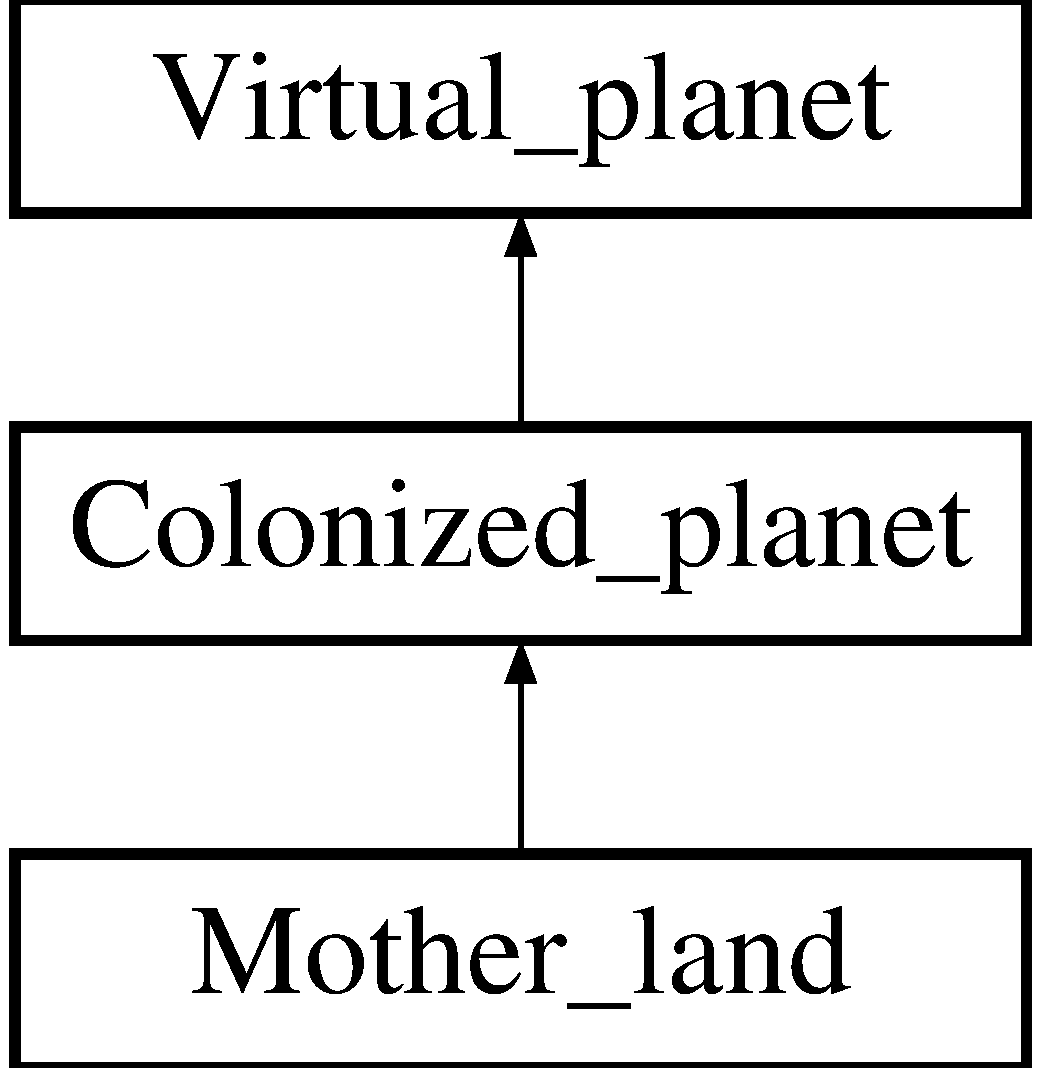
\includegraphics[height=3.000000cm]{classColonized__planet}
\end{center}
\end{figure}
\subsection*{Fonctions membres publiques}
\begin{DoxyCompactItemize}
\item 
\hyperlink{classColonized__planet_a06b9d86c2d48d101688ec202c8d37dd8}{Colonized\-\_\-planet} (\hyperlink{classWorld}{World} \&, unsigned, unsigned, \hyperlink{classFaction}{Faction} \&)
\begin{DoxyCompactList}\small\item\em Constructeur, prépare la planète. \end{DoxyCompactList}\item 
\hyperlink{classColonized__planet_a39273e5d94de78e93438e5007ddbecc1}{Colonized\-\_\-planet} (\hyperlink{classVirtual__planet}{Virtual\-\_\-planet} $\ast$, \hyperlink{classFaction}{Faction} \&)
\begin{DoxyCompactList}\small\item\em Création d'une planète colonisée à partir d'une autre planète. \end{DoxyCompactList}\item 
void \hyperlink{classColonized__planet_ac4f99490dc15c7715c1b476a490228a4}{update\-\_\-neighbourhood} (\hyperlink{classVirtual__planet}{Virtual\-\_\-planet} $\ast$, \hyperlink{classVirtual__planet}{Virtual\-\_\-planet} $\ast$)
\begin{DoxyCompactList}\small\item\em Mise à jour du voisinage. \end{DoxyCompactList}\item 
bool \hyperlink{classColonized__planet_a7a0ca9e84837a2f03900f01b1e1a3fa6}{attack} (\hyperlink{classVirtual__planet}{Virtual\-\_\-planet} $\ast$)
\begin{DoxyCompactList}\small\item\em Attaque une planète. \end{DoxyCompactList}\item 
virtual bool \hyperlink{classColonized__planet_af637772fb84e45bb47447c88aa8d3f4a}{is\-\_\-attacked} (\hyperlink{classVirtual__planet}{Virtual\-\_\-planet} $\ast$)
\begin{DoxyCompactList}\small\item\em La planète est attaquée. \end{DoxyCompactList}\item 
void \hyperlink{classColonized__planet_ae05d410995da1c4846bee779a3f6c831}{convert\-\_\-to\-\_\-free\-\_\-planet} ()
\begin{DoxyCompactList}\small\item\em Transforme la colonie courante en free planete. \end{DoxyCompactList}\item 
\hyperlink{classFaction}{Faction} \& \hyperlink{classColonized__planet_a78748eadea1186e104ccc247a1d1f546}{get\-\_\-faction} ()
\begin{DoxyCompactList}\small\item\em \hyperlink{classFaction}{Faction} à laquelle appartient la planète. \end{DoxyCompactList}\item 
double \hyperlink{classColonized__planet_a587ca19477274169b045a94c1dd186a3}{get\-\_\-defense} ()
\begin{DoxyCompactList}\small\item\em Défense totale de la planète. \end{DoxyCompactList}\item 
double \hyperlink{classColonized__planet_a167b41cbb51c1d19d40cb3707af2ea59}{get\-\_\-production} ()
\begin{DoxyCompactList}\small\item\em Production de la planète. \end{DoxyCompactList}\item 
\hypertarget{classColonized__planet_a6739ad553640a6b5a02dfd9d97e7ba2d}{\hyperlink{classVirtual__planet}{Virtual\-\_\-planet} $\ast$ {\bfseries get\-\_\-target} ()}\label{classColonized__planet_a6739ad553640a6b5a02dfd9d97e7ba2d}

\item 
void \hyperlink{classColonized__planet_a0b5f60dc9483575db786313282e29886}{demand\-\_\-to\-\_\-faction} (double)
\begin{DoxyCompactList}\small\item\em Réalise une demande de fonds auprès de la faction. \end{DoxyCompactList}\item 
double \hyperlink{classColonized__planet_aa6f348f353079fb347dc8ac09d8b1067}{estimate\-\_\-cost} ()
\begin{DoxyCompactList}\small\item\em Estime le coût d'une attaque. \end{DoxyCompactList}\item 
void \hyperlink{classColonized__planet_a35968145bd39bba554c026e499976e44}{add\-\_\-to\-\_\-budget} (double)
\begin{DoxyCompactList}\small\item\em Ajoute les fonds obtenus auprès de la faction. \end{DoxyCompactList}\item 
\hypertarget{classColonized__planet_a61098b25c33cbf5bf36e3629a42f7ee7}{void \hyperlink{classColonized__planet_a61098b25c33cbf5bf36e3629a42f7ee7}{reinitialisate\-\_\-target} ()}\label{classColonized__planet_a61098b25c33cbf5bf36e3629a42f7ee7}

\begin{DoxyCompactList}\small\item\em Réinitialise la cible, annule la tentative d'attaque. \end{DoxyCompactList}\item 
\hypertarget{classColonized__planet_a1d3897c8ef1772fa9908fee7c5830f77}{char \hyperlink{classColonized__planet_a1d3897c8ef1772fa9908fee7c5830f77}{display} ()}\label{classColonized__planet_a1d3897c8ef1772fa9908fee7c5830f77}

\begin{DoxyCompactList}\small\item\em Caractère par défaut (point) \end{DoxyCompactList}\item 
\hypertarget{classColonized__planet_af8e3c6d3e72bf80b2e44013ceba2087f}{std\-::string \hyperlink{classColonized__planet_af8e3c6d3e72bf80b2e44013ceba2087f}{get\-\_\-color\-\_\-name} ()}\label{classColonized__planet_af8e3c6d3e72bf80b2e44013ceba2087f}

\begin{DoxyCompactList}\small\item\em Couleur par défaut (gris) \end{DoxyCompactList}\item 
void \hyperlink{classColonized__planet_ab8d7c5d4c58fed9239277f18b9de174a}{run} ()
\begin{DoxyCompactList}\small\item\em Joue le tour. \end{DoxyCompactList}\item 
\hypertarget{classColonized__planet_ad364c3baffd5ad81d3208b1228cc35e4}{bool \hyperlink{classColonized__planet_ad364c3baffd5ad81d3208b1228cc35e4}{can\-\_\-be\-\_\-replaced} ()}\label{classColonized__planet_ad364c3baffd5ad81d3208b1228cc35e4}

\begin{DoxyCompactList}\small\item\em Renvoie true si la planete n'est pas un agent. \end{DoxyCompactList}\end{DoxyCompactItemize}
\subsection*{Attributs protégés}
\begin{DoxyCompactItemize}
\item 
\hypertarget{classColonized__planet_ac645c006479bc9722dc3df7de53613bb}{double \hyperlink{classColonized__planet_ac645c006479bc9722dc3df7de53613bb}{colony\-\_\-defense\-\_\-}}\label{classColonized__planet_ac645c006479bc9722dc3df7de53613bb}

\begin{DoxyCompactList}\small\item\em Valeur de défense. \end{DoxyCompactList}\item 
\hypertarget{classColonized__planet_affcfbff793cae417ce77ab90b4868ef8}{double \hyperlink{classColonized__planet_affcfbff793cae417ce77ab90b4868ef8}{colony\-\_\-production\-\_\-}}\label{classColonized__planet_affcfbff793cae417ce77ab90b4868ef8}

\begin{DoxyCompactList}\small\item\em Valeur de production de monnaie. \end{DoxyCompactList}\item 
\hypertarget{classColonized__planet_a0f362a09eaf2da16c442decbdaf57d21}{\hyperlink{classFaction}{Faction} \& \hyperlink{classColonized__planet_a0f362a09eaf2da16c442decbdaf57d21}{faction\-\_\-}}\label{classColonized__planet_a0f362a09eaf2da16c442decbdaf57d21}

\begin{DoxyCompactList}\small\item\em \hyperlink{classFaction}{Faction} à laquelle appartient la colonie. \end{DoxyCompactList}\item 
\hypertarget{classColonized__planet_af24d15905b14b8a1af9c202791dffe5f}{\hyperlink{classVirtual__planet}{Virtual\-\_\-planet} $\ast$ \hyperlink{classColonized__planet_af24d15905b14b8a1af9c202791dffe5f}{target\-\_\-}}\label{classColonized__planet_af24d15905b14b8a1af9c202791dffe5f}

\begin{DoxyCompactList}\small\item\em Planète ciblée par une éventuelle attaque. \end{DoxyCompactList}\item 
\hypertarget{classColonized__planet_a9ba08dc04733fcef48b1107ec8b6af84}{double \hyperlink{classColonized__planet_a9ba08dc04733fcef48b1107ec8b6af84}{budget\-\_\-}}\label{classColonized__planet_a9ba08dc04733fcef48b1107ec8b6af84}

\begin{DoxyCompactList}\small\item\em Argent disponible. \end{DoxyCompactList}\item 
\hypertarget{classColonized__planet_af5c7aba0db9f3a8c28d25a309c79ca23}{double \hyperlink{classColonized__planet_af5c7aba0db9f3a8c28d25a309c79ca23}{demand\-\_\-}}\label{classColonized__planet_af5c7aba0db9f3a8c28d25a309c79ca23}

\begin{DoxyCompactList}\small\item\em Coût estimé d'une opération. \end{DoxyCompactList}\end{DoxyCompactItemize}
\subsection*{Attributs protégés statiques}
\begin{DoxyCompactItemize}
\item 
\hypertarget{classColonized__planet_acb5d3542a5441019bcba92197119617c}{static const int \hyperlink{classColonized__planet_acb5d3542a5441019bcba92197119617c}{M\-A\-X\-\_\-\-C\-O\-L\-O\-N\-Y\-\_\-\-D\-E\-F\-E\-N\-S\-E} = 50}\label{classColonized__planet_acb5d3542a5441019bcba92197119617c}

\begin{DoxyCompactList}\small\item\em Valeur de défense maximum. \end{DoxyCompactList}\item 
\hypertarget{classColonized__planet_a8521f4f3a3d0431932cdd2e1988b358f}{static const int \hyperlink{classColonized__planet_a8521f4f3a3d0431932cdd2e1988b358f}{M\-A\-X\-\_\-\-C\-O\-L\-O\-N\-Y\-\_\-\-P\-R\-O\-D\-U\-C\-T\-I\-O\-N} = 15}\label{classColonized__planet_a8521f4f3a3d0431932cdd2e1988b358f}

\begin{DoxyCompactList}\small\item\em Valeur de production maximum. \end{DoxyCompactList}\item 
\hypertarget{classColonized__planet_af44fcc5ced3d38fc514d5daf0abea01d}{static const int \hyperlink{classColonized__planet_af44fcc5ced3d38fc514d5daf0abea01d}{C\-O\-L\-O\-N\-Y\-\_\-\-M\-U\-L\-T\-I\-P\-L\-I\-C\-A\-T\-O\-R} = 10}\label{classColonized__planet_af44fcc5ced3d38fc514d5daf0abea01d}

\begin{DoxyCompactList}\small\item\em Facteur de production. \end{DoxyCompactList}\end{DoxyCompactItemize}
\subsection*{Membres hérités additionnels}


\subsection{Description détaillée}
Planète colonisée. 

Une planète colonisée est une planète possédée par une faction 

\subsection{Documentation des constructeurs et destructeur}
\hypertarget{classColonized__planet_a06b9d86c2d48d101688ec202c8d37dd8}{\index{Colonized\-\_\-planet@{Colonized\-\_\-planet}!Colonized\-\_\-planet@{Colonized\-\_\-planet}}
\index{Colonized\-\_\-planet@{Colonized\-\_\-planet}!Colonized_planet@{Colonized\-\_\-planet}}
\subsubsection[{Colonized\-\_\-planet}]{\setlength{\rightskip}{0pt plus 5cm}Colonized\-\_\-planet\-::\-Colonized\-\_\-planet (
\begin{DoxyParamCaption}
\item[{{\bf World} \&}]{world, }
\item[{unsigned}]{pos\-\_\-x, }
\item[{unsigned}]{pos\-\_\-y, }
\item[{{\bf Faction} \&}]{fac}
\end{DoxyParamCaption}
)}}\label{classColonized__planet_a06b9d86c2d48d101688ec202c8d37dd8}


Constructeur, prépare la planète. 

Met à jour la liste des agents en attente et ajoute la planète à la liste des colonies de la faction.


\begin{DoxyParams}{Paramètres}
{\em world} & plateau de jeu \\
\hline
{\em pos\-\_\-x} & numéro de la ligne sur la grille \\
\hline
{\em pos\-\_\-y} & numéro de la colonne sur la grille \\
\hline
{\em fac} & faction à laquelle doit appartenir la nouvelle planète \\
\hline
\end{DoxyParams}
\hypertarget{classColonized__planet_a39273e5d94de78e93438e5007ddbecc1}{\index{Colonized\-\_\-planet@{Colonized\-\_\-planet}!Colonized\-\_\-planet@{Colonized\-\_\-planet}}
\index{Colonized\-\_\-planet@{Colonized\-\_\-planet}!Colonized_planet@{Colonized\-\_\-planet}}
\subsubsection[{Colonized\-\_\-planet}]{\setlength{\rightskip}{0pt plus 5cm}Colonized\-\_\-planet\-::\-Colonized\-\_\-planet (
\begin{DoxyParamCaption}
\item[{{\bf Virtual\-\_\-planet} $\ast$}]{fp, }
\item[{{\bf Faction} \&}]{faction}
\end{DoxyParamCaption}
)}}\label{classColonized__planet_a39273e5d94de78e93438e5007ddbecc1}


Création d'une planète colonisée à partir d'une autre planète. 


\begin{DoxyParams}{Paramètres}
{\em fp} & planète d'origine \\
\hline
{\em faction} & faction à laquelle doit appartenir la nouvelle planète\\
\hline
\end{DoxyParams}
\begin{DoxyNote}{Note}
Tient compte du voisinage de l'ancienne planète et le met à jour 
\end{DoxyNote}


\subsection{Documentation des fonctions membres}
\hypertarget{classColonized__planet_a35968145bd39bba554c026e499976e44}{\index{Colonized\-\_\-planet@{Colonized\-\_\-planet}!add\-\_\-to\-\_\-budget@{add\-\_\-to\-\_\-budget}}
\index{add\-\_\-to\-\_\-budget@{add\-\_\-to\-\_\-budget}!Colonized_planet@{Colonized\-\_\-planet}}
\subsubsection[{add\-\_\-to\-\_\-budget}]{\setlength{\rightskip}{0pt plus 5cm}void Colonized\-\_\-planet\-::add\-\_\-to\-\_\-budget (
\begin{DoxyParamCaption}
\item[{double}]{given\-\_\-money}
\end{DoxyParamCaption}
)}}\label{classColonized__planet_a35968145bd39bba554c026e499976e44}


Ajoute les fonds obtenus auprès de la faction. 

Augmente le budget du montant obtenu, et diminue d'autant la demande précédemment effectuée.


\begin{DoxyParams}{Paramètres}
{\em given\-\_\-money} & Montant obtenu \\
\hline
\end{DoxyParams}
\hypertarget{classColonized__planet_a7a0ca9e84837a2f03900f01b1e1a3fa6}{\index{Colonized\-\_\-planet@{Colonized\-\_\-planet}!attack@{attack}}
\index{attack@{attack}!Colonized_planet@{Colonized\-\_\-planet}}
\subsubsection[{attack}]{\setlength{\rightskip}{0pt plus 5cm}bool Colonized\-\_\-planet\-::attack (
\begin{DoxyParamCaption}
\item[{{\bf Virtual\-\_\-planet} $\ast$}]{victim}
\end{DoxyParamCaption}
)}}\label{classColonized__planet_a7a0ca9e84837a2f03900f01b1e1a3fa6}


Attaque une planète. 


\begin{DoxyParams}{Paramètres}
{\em victim} & planète qui est attaquée \\
\hline
\end{DoxyParams}
\begin{DoxyReturn}{Renvoie}
victoire de l'attaque 
\end{DoxyReturn}
\hypertarget{classColonized__planet_ae05d410995da1c4846bee779a3f6c831}{\index{Colonized\-\_\-planet@{Colonized\-\_\-planet}!convert\-\_\-to\-\_\-free\-\_\-planet@{convert\-\_\-to\-\_\-free\-\_\-planet}}
\index{convert\-\_\-to\-\_\-free\-\_\-planet@{convert\-\_\-to\-\_\-free\-\_\-planet}!Colonized_planet@{Colonized\-\_\-planet}}
\subsubsection[{convert\-\_\-to\-\_\-free\-\_\-planet}]{\setlength{\rightskip}{0pt plus 5cm}void Colonized\-\_\-planet\-::convert\-\_\-to\-\_\-free\-\_\-planet (
\begin{DoxyParamCaption}
{}
\end{DoxyParamCaption}
)}}\label{classColonized__planet_ae05d410995da1c4846bee779a3f6c831}


Transforme la colonie courante en free planete. 

\begin{DoxyWarning}{Avertissement}
Ne supprime pas la colonie et ne met pas a jour le voisinage !! 
\end{DoxyWarning}
\hypertarget{classColonized__planet_a0b5f60dc9483575db786313282e29886}{\index{Colonized\-\_\-planet@{Colonized\-\_\-planet}!demand\-\_\-to\-\_\-faction@{demand\-\_\-to\-\_\-faction}}
\index{demand\-\_\-to\-\_\-faction@{demand\-\_\-to\-\_\-faction}!Colonized_planet@{Colonized\-\_\-planet}}
\subsubsection[{demand\-\_\-to\-\_\-faction}]{\setlength{\rightskip}{0pt plus 5cm}void Colonized\-\_\-planet\-::demand\-\_\-to\-\_\-faction (
\begin{DoxyParamCaption}
\item[{double}]{cost}
\end{DoxyParamCaption}
)}}\label{classColonized__planet_a0b5f60dc9483575db786313282e29886}


Réalise une demande de fonds auprès de la faction. 


\begin{DoxyParams}{Paramètres}
{\em cost} & Montant demandé \\
\hline
\end{DoxyParams}
\hypertarget{classColonized__planet_aa6f348f353079fb347dc8ac09d8b1067}{\index{Colonized\-\_\-planet@{Colonized\-\_\-planet}!estimate\-\_\-cost@{estimate\-\_\-cost}}
\index{estimate\-\_\-cost@{estimate\-\_\-cost}!Colonized_planet@{Colonized\-\_\-planet}}
\subsubsection[{estimate\-\_\-cost}]{\setlength{\rightskip}{0pt plus 5cm}double Colonized\-\_\-planet\-::estimate\-\_\-cost (
\begin{DoxyParamCaption}
{}
\end{DoxyParamCaption}
)\hspace{0.3cm}{\ttfamily [virtual]}}}\label{classColonized__planet_aa6f348f353079fb347dc8ac09d8b1067}


Estime le coût d'une attaque. 

\begin{DoxyReturn}{Renvoie}
coût estimé 
\end{DoxyReturn}


Réimplémentée à partir de \hyperlink{classVirtual__planet_a7f442fee301927b27217877abb765833}{Virtual\-\_\-planet}.

\hypertarget{classColonized__planet_a587ca19477274169b045a94c1dd186a3}{\index{Colonized\-\_\-planet@{Colonized\-\_\-planet}!get\-\_\-defense@{get\-\_\-defense}}
\index{get\-\_\-defense@{get\-\_\-defense}!Colonized_planet@{Colonized\-\_\-planet}}
\subsubsection[{get\-\_\-defense}]{\setlength{\rightskip}{0pt plus 5cm}double Colonized\-\_\-planet\-::get\-\_\-defense (
\begin{DoxyParamCaption}
{}
\end{DoxyParamCaption}
)\hspace{0.3cm}{\ttfamily [virtual]}}}\label{classColonized__planet_a587ca19477274169b045a94c1dd186a3}


Défense totale de la planète. 

\begin{DoxyReturn}{Renvoie}
somme de la défense naturelle de la planète et de celle de la colonie 
\end{DoxyReturn}


Réimplémentée à partir de \hyperlink{classVirtual__planet_a25045d61c5ee29b94de56db88fa96f98}{Virtual\-\_\-planet}.

\hypertarget{classColonized__planet_a78748eadea1186e104ccc247a1d1f546}{\index{Colonized\-\_\-planet@{Colonized\-\_\-planet}!get\-\_\-faction@{get\-\_\-faction}}
\index{get\-\_\-faction@{get\-\_\-faction}!Colonized_planet@{Colonized\-\_\-planet}}
\subsubsection[{get\-\_\-faction}]{\setlength{\rightskip}{0pt plus 5cm}{\bf Faction} \& Colonized\-\_\-planet\-::get\-\_\-faction (
\begin{DoxyParamCaption}
{}
\end{DoxyParamCaption}
)\hspace{0.3cm}{\ttfamily [virtual]}}}\label{classColonized__planet_a78748eadea1186e104ccc247a1d1f546}


\hyperlink{classFaction}{Faction} à laquelle appartient la planète. 

\begin{DoxyReturn}{Renvoie}
faction 
\end{DoxyReturn}


Réimplémentée à partir de \hyperlink{classVirtual__planet_ac0d0e30029566b9113652c04ec2e6599}{Virtual\-\_\-planet}.

\hypertarget{classColonized__planet_a167b41cbb51c1d19d40cb3707af2ea59}{\index{Colonized\-\_\-planet@{Colonized\-\_\-planet}!get\-\_\-production@{get\-\_\-production}}
\index{get\-\_\-production@{get\-\_\-production}!Colonized_planet@{Colonized\-\_\-planet}}
\subsubsection[{get\-\_\-production}]{\setlength{\rightskip}{0pt plus 5cm}double Colonized\-\_\-planet\-::get\-\_\-production (
\begin{DoxyParamCaption}
{}
\end{DoxyParamCaption}
)\hspace{0.3cm}{\ttfamily [virtual]}}}\label{classColonized__planet_a167b41cbb51c1d19d40cb3707af2ea59}


Production de la planète. 

\begin{DoxyReturn}{Renvoie}
somme de la production naturelle de la planète et de celle de la colonie 
\end{DoxyReturn}


Réimplémentée à partir de \hyperlink{classVirtual__planet_a4294d3312671d720dca0b72a1648e6a4}{Virtual\-\_\-planet}.

\hypertarget{classColonized__planet_af637772fb84e45bb47447c88aa8d3f4a}{\index{Colonized\-\_\-planet@{Colonized\-\_\-planet}!is\-\_\-attacked@{is\-\_\-attacked}}
\index{is\-\_\-attacked@{is\-\_\-attacked}!Colonized_planet@{Colonized\-\_\-planet}}
\subsubsection[{is\-\_\-attacked}]{\setlength{\rightskip}{0pt plus 5cm}bool Colonized\-\_\-planet\-::is\-\_\-attacked (
\begin{DoxyParamCaption}
\item[{{\bf Virtual\-\_\-planet} $\ast$}]{attacker}
\end{DoxyParamCaption}
)\hspace{0.3cm}{\ttfamily [virtual]}}}\label{classColonized__planet_af637772fb84e45bb47447c88aa8d3f4a}


La planète est attaquée. 

Lorsque la planète est attaquée, elle tente de parer l'attaque. Son score de défense est utilisé et peut être inpacté ainsi que la valeur de production.


\begin{DoxyParams}{Paramètres}
{\em attacker} & planète offensive \\
\hline
\end{DoxyParams}
\begin{DoxyReturn}{Renvoie}
victoire de l'attaque
\end{DoxyReturn}
\begin{DoxyNote}{Note}
Si la planète ne parvient pas à parer l'attaque alors elle est éliminée de la liste d'attente de jeu car elle sera supprimée par la suite.
\end{DoxyNote}
\begin{DoxySeeAlso}{Voir également}
\hyperlink{classColonized__planet_affcfbff793cae417ce77ab90b4868ef8}{colony\-\_\-production\-\_\-} 

\hyperlink{classColonized__planet_ac645c006479bc9722dc3df7de53613bb}{colony\-\_\-defense\-\_\-} 
\end{DoxySeeAlso}


Réimplémentée à partir de \hyperlink{classVirtual__planet_aa0712e85ae6ae7e9f05bd6d943a1a7b4}{Virtual\-\_\-planet}.



Réimplémentée dans \hyperlink{classMother__land_a295325cdedbfcfb17c200a4a7438761c}{Mother\-\_\-land}.

\hypertarget{classColonized__planet_ab8d7c5d4c58fed9239277f18b9de174a}{\index{Colonized\-\_\-planet@{Colonized\-\_\-planet}!run@{run}}
\index{run@{run}!Colonized_planet@{Colonized\-\_\-planet}}
\subsubsection[{run}]{\setlength{\rightskip}{0pt plus 5cm}void Colonized\-\_\-planet\-::run (
\begin{DoxyParamCaption}
{}
\end{DoxyParamCaption}
)}}\label{classColonized__planet_ab8d7c5d4c58fed9239277f18b9de174a}


Joue le tour. 

La planète peut choisir d'attaquer ou bien de produire des richesses.

\begin{DoxyReturn}{Renvoie}
Booléen indiquant si la planète a réalisé une attaque 
\end{DoxyReturn}
\hypertarget{classColonized__planet_ac4f99490dc15c7715c1b476a490228a4}{\index{Colonized\-\_\-planet@{Colonized\-\_\-planet}!update\-\_\-neighbourhood@{update\-\_\-neighbourhood}}
\index{update\-\_\-neighbourhood@{update\-\_\-neighbourhood}!Colonized_planet@{Colonized\-\_\-planet}}
\subsubsection[{update\-\_\-neighbourhood}]{\setlength{\rightskip}{0pt plus 5cm}void Colonized\-\_\-planet\-::update\-\_\-neighbourhood (
\begin{DoxyParamCaption}
\item[{{\bf Virtual\-\_\-planet} $\ast$}]{old\-\_\-one, }
\item[{{\bf Virtual\-\_\-planet} $\ast$}]{new\-\_\-one}
\end{DoxyParamCaption}
)\hspace{0.3cm}{\ttfamily [virtual]}}}\label{classColonized__planet_ac4f99490dc15c7715c1b476a490228a4}


Mise à jour du voisinage. 

Parcourt le voisinage de la planète courante et remplace old\-\_\-one par new\-\_\-one dans la liste.


\begin{DoxyParams}{Paramètres}
{\em old\-\_\-one} & ancienne planète \\
\hline
{\em new\-\_\-one} & nouvelle planète\\
\hline
\end{DoxyParams}
\begin{DoxyNote}{Note}
Si l'ancienne planète était la cible de l'un des voisins, alors cette cible est effacée. 
\end{DoxyNote}


Réimplémentée à partir de \hyperlink{classVirtual__planet_ac67c164e630df471819336d2404a99af}{Virtual\-\_\-planet}.



La documentation de cette classe a été générée à partir des fichiers suivants \-:\begin{DoxyCompactItemize}
\item 
/home/pipissavy/\-Dropbox/\-Cours/\-I\-S\-I\-M\-A/\-Z\-Z2/simulation/simu\-\_\-multi\-\_\-agents/src/Colonized\-\_\-planet.\-hpp\item 
/home/pipissavy/\-Dropbox/\-Cours/\-I\-S\-I\-M\-A/\-Z\-Z2/simulation/simu\-\_\-multi\-\_\-agents/src/Colonized\-\_\-planet.\-cpp\end{DoxyCompactItemize}

\hypertarget{classComparator}{\section{Référence de la classe Comparator}
\label{classComparator}\index{Comparator@{Comparator}}
}


Comparateur de planètes colonisées.  




{\ttfamily \#include $<$Faction.\-hpp$>$}

\subsection*{Fonctions membres publiques}
\begin{DoxyCompactItemize}
\item 
\hyperlink{classComparator_aff716639b83e77e710f3c3175c4b43d0}{Comparator} (\hyperlink{classColonized__planet}{Colonized\-\_\-planet} $\ast$colonized\-\_\-planet)
\begin{DoxyCompactList}\small\item\em Constructeur. \end{DoxyCompactList}\item 
bool \hyperlink{classComparator_aa063882ba2357118b02cd4e01d807480}{operator()} (std\-::pair$<$ \hyperlink{classColonized__planet}{Colonized\-\_\-planet} $\ast$, double $>$ pair\-\_\-colony)
\begin{DoxyCompactList}\small\item\em Comparaison avec la planète de base. \end{DoxyCompactList}\end{DoxyCompactItemize}
\subsection*{Attributs privés}
\begin{DoxyCompactItemize}
\item 
\hypertarget{classComparator_a5b42c2a1661147200983835ac36802cf}{\hyperlink{classColonized__planet}{Colonized\-\_\-planet} $\ast$ \hyperlink{classComparator_a5b42c2a1661147200983835ac36802cf}{colonized\-\_\-planet\-\_\-}}\label{classComparator_a5b42c2a1661147200983835ac36802cf}

\begin{DoxyCompactList}\small\item\em Planète qui doit servir de base pour la comparaison. \end{DoxyCompactList}\end{DoxyCompactItemize}


\subsection{Description détaillée}
Comparateur de planètes colonisées. 

\subsection{Documentation des constructeurs et destructeur}
\hypertarget{classComparator_aff716639b83e77e710f3c3175c4b43d0}{\index{Comparator@{Comparator}!Comparator@{Comparator}}
\index{Comparator@{Comparator}!Comparator@{Comparator}}
\subsubsection[{Comparator}]{\setlength{\rightskip}{0pt plus 5cm}Comparator\-::\-Comparator (
\begin{DoxyParamCaption}
\item[{{\bf Colonized\-\_\-planet} $\ast$}]{colonized\-\_\-planet}
\end{DoxyParamCaption}
)\hspace{0.3cm}{\ttfamily [inline]}}}\label{classComparator_aff716639b83e77e710f3c3175c4b43d0}


Constructeur. 


\begin{DoxyParams}{Paramètres}
{\em colonized\-\_\-planet} & planète servant d'élément de comparaison \\
\hline
\end{DoxyParams}


\subsection{Documentation des fonctions membres}
\hypertarget{classComparator_aa063882ba2357118b02cd4e01d807480}{\index{Comparator@{Comparator}!operator()@{operator()}}
\index{operator()@{operator()}!Comparator@{Comparator}}
\subsubsection[{operator()}]{\setlength{\rightskip}{0pt plus 5cm}bool Comparator\-::operator() (
\begin{DoxyParamCaption}
\item[{std\-::pair$<$ {\bf Colonized\-\_\-planet} $\ast$, double $>$}]{pair\-\_\-colony}
\end{DoxyParamCaption}
)\hspace{0.3cm}{\ttfamily [inline]}}}\label{classComparator_aa063882ba2357118b02cd4e01d807480}


Comparaison avec la planète de base. 


\begin{DoxyParams}{Paramètres}
{\em pair\-\_\-colony} & une paire dont le premier membre est comparé avec la planète de base \\
\hline
\end{DoxyParams}
\begin{DoxyReturn}{Renvoie}
Booléen à vrai si la comparaison est valide 
\end{DoxyReturn}


La documentation de cette classe a été générée à partir du fichier suivant \-:\begin{DoxyCompactItemize}
\item 
/home/pipissavy/\-Dropbox/\-Cours/\-I\-S\-I\-M\-A/\-Z\-Z2/simulation/simu\-\_\-multi\-\_\-agents/src/Faction.\-hpp\end{DoxyCompactItemize}

\hypertarget{classDisplayer}{\section{Référence de la classe Displayer}
\label{classDisplayer}\index{Displayer@{Displayer}}
}


Zone d'affichage de l'application.  




{\ttfamily \#include $<$displayer.\-h$>$}

Graphe d'héritage de Displayer\-:\begin{figure}[H]
\begin{center}
\leavevmode
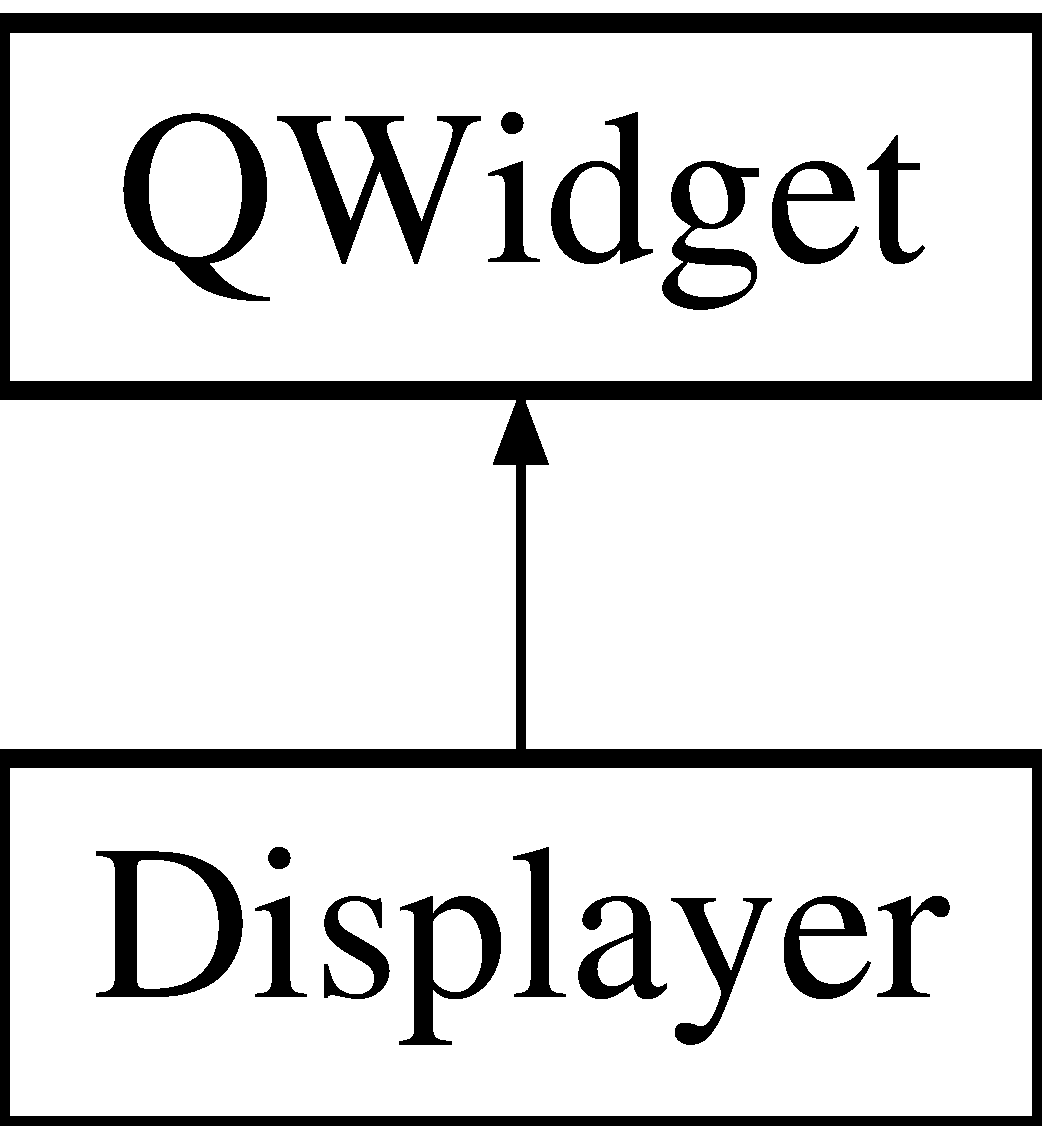
\includegraphics[height=2.000000cm]{classDisplayer}
\end{center}
\end{figure}
\subsection*{Fonctions membres publiques}
\begin{DoxyCompactItemize}
\item 
\hyperlink{classDisplayer_a04104e09562ed9f64a96174ab5409dc2}{Displayer} (Q\-Widget $\ast$parent=0)
\begin{DoxyCompactList}\small\item\em Constructeur par défaut. \end{DoxyCompactList}\item 
\hyperlink{classDisplayer_a099a08baae9c7985acf6cca4fa2d0509}{Displayer} (Q\-Main\-Window $\ast$)
\begin{DoxyCompactList}\small\item\em Crée l'interface visuelle de présentation de la grille de simulation. \end{DoxyCompactList}\item 
void \hyperlink{classDisplayer_a06d6e9b18c26c121d21d95bb5a352ee0}{afficher\-Rect} ()
\item 
\hypertarget{classDisplayer_a43b024cbfed7610ee3b91a7ba52a1a5b}{void \hyperlink{classDisplayer_a43b024cbfed7610ee3b91a7ba52a1a5b}{display\-\_\-world} ()}\label{classDisplayer_a43b024cbfed7610ee3b91a7ba52a1a5b}

\begin{DoxyCompactList}\small\item\em Affiche la grille. \end{DoxyCompactList}\item 
bool \hyperlink{classDisplayer_a60656ce57ab16d1265fea3dfa5bf22cf}{play} ()
\begin{DoxyCompactList}\small\item\em Teste si la partie n'est pas finie. \end{DoxyCompactList}\item 
\hypertarget{classDisplayer_a9f5cdcdfae1594e835973926df0da537}{\hyperlink{classDisplayer_a9f5cdcdfae1594e835973926df0da537}{$\sim$\-Displayer} ()}\label{classDisplayer_a9f5cdcdfae1594e835973926df0da537}

\begin{DoxyCompactList}\small\item\em Supprime et nettoie l'interface visuelle de présentation de la grille de simulation. \end{DoxyCompactList}\end{DoxyCompactItemize}
\subsection*{Connecteurs protégés}
\begin{DoxyCompactItemize}
\item 
\hypertarget{classDisplayer_a560b41e509deb82d5ae56b5ff60e093c}{void \hyperlink{classDisplayer_a560b41e509deb82d5ae56b5ff60e093c}{timer\-Event} ()}\label{classDisplayer_a560b41e509deb82d5ae56b5ff60e093c}

\begin{DoxyCompactList}\small\item\em Evènement de mise à jour de l'affichage. \end{DoxyCompactList}\item 
\hypertarget{classDisplayer_a557745fd320fb608f4067ea3fcbf3a56}{void \hyperlink{classDisplayer_a557745fd320fb608f4067ea3fcbf3a56}{refresh} ()}\label{classDisplayer_a557745fd320fb608f4067ea3fcbf3a56}

\begin{DoxyCompactList}\small\item\em Commande de rafraichissement de l'affichage. \end{DoxyCompactList}\end{DoxyCompactItemize}
\subsection*{Fonctions membres privées}
\begin{DoxyCompactItemize}
\item 
\hypertarget{classDisplayer_a64736a6c3bf40f87fb54562dcdb51b21}{void \hyperlink{classDisplayer_a64736a6c3bf40f87fb54562dcdb51b21}{end} ()}\label{classDisplayer_a64736a6c3bf40f87fb54562dcdb51b21}

\begin{DoxyCompactList}\small\item\em Affiche la faction gagnante dans une boîte à message. \end{DoxyCompactList}\item 
void \hyperlink{classDisplayer_a4b66ff00950bc1d57bffa61a767c0303}{display\-\_\-planet} (unsigned pos\-X, unsigned pos\-Y)
\begin{DoxyCompactList}\small\item\em Affiche une planète. \end{DoxyCompactList}\end{DoxyCompactItemize}
\subsection*{Attributs privés}
\begin{DoxyCompactItemize}
\item 
\hypertarget{classDisplayer_a2b3b84d51d4bb077d52ede2a2abc6191}{Q\-Graphics\-Scene $\ast$ \hyperlink{classDisplayer_a2b3b84d51d4bb077d52ede2a2abc6191}{m\-\_\-scene}}\label{classDisplayer_a2b3b84d51d4bb077d52ede2a2abc6191}

\begin{DoxyCompactList}\small\item\em Scène de l'affichage. \end{DoxyCompactList}\item 
\hypertarget{classDisplayer_a793b9f323b4d24428f1376528b537515}{Q\-Graphics\-View $\ast$ \hyperlink{classDisplayer_a793b9f323b4d24428f1376528b537515}{m\-\_\-view}}\label{classDisplayer_a793b9f323b4d24428f1376528b537515}

\begin{DoxyCompactList}\small\item\em Vue. \end{DoxyCompactList}\item 
\hypertarget{classDisplayer_acf5e0801f0353ad1300ea901f8038fb5}{\hyperlink{classWorld}{World} \hyperlink{classDisplayer_acf5e0801f0353ad1300ea901f8038fb5}{world\-\_\-}}\label{classDisplayer_acf5e0801f0353ad1300ea901f8038fb5}

\begin{DoxyCompactList}\small\item\em Plateau de jeu. \end{DoxyCompactList}\item 
\hypertarget{classDisplayer_abf6048109c2f782b47932babc1c72b79}{unsigned \hyperlink{classDisplayer_abf6048109c2f782b47932babc1c72b79}{size\-\_\-planete\-\_\-}}\label{classDisplayer_abf6048109c2f782b47932babc1c72b79}

\begin{DoxyCompactList}\small\item\em Taille d'une planète à l'affichage (px) \end{DoxyCompactList}\item 
\hypertarget{classDisplayer_aedcdc7b40771c068fb70f9f74b2d6689}{unsigned \hyperlink{classDisplayer_aedcdc7b40771c068fb70f9f74b2d6689}{len\-\_\-text\-\_\-box\-\_\-}}\label{classDisplayer_aedcdc7b40771c068fb70f9f74b2d6689}

\begin{DoxyCompactList}\small\item\em Largeur du panneau latéral (px) \end{DoxyCompactList}\item 
\hypertarget{classDisplayer_aff59f7de619d0d84e91aaf6087b55ebc}{unsigned \hyperlink{classDisplayer_aff59f7de619d0d84e91aaf6087b55ebc}{len\-\_\-canvas\-\_\-}}\label{classDisplayer_aff59f7de619d0d84e91aaf6087b55ebc}

\begin{DoxyCompactList}\small\item\em Largeur du panneau graphique (px) \end{DoxyCompactList}\item 
\hypertarget{classDisplayer_ae7d9e96ca745d502672369fc4d1cde5c}{unsigned \hyperlink{classDisplayer_ae7d9e96ca745d502672369fc4d1cde5c}{hei\-\_\-canvas\-\_\-}}\label{classDisplayer_ae7d9e96ca745d502672369fc4d1cde5c}

\begin{DoxyCompactList}\small\item\em Hauteur du panneau graphique (px) \end{DoxyCompactList}\item 
\hypertarget{classDisplayer_a9edd62c6f4cf550385c1dc9933e49d0e}{Q\-Timer $\ast$ \hyperlink{classDisplayer_a9edd62c6f4cf550385c1dc9933e49d0e}{timer}}\label{classDisplayer_a9edd62c6f4cf550385c1dc9933e49d0e}

\begin{DoxyCompactList}\small\item\em Chronomètre pour gérer la fréquence d'affichage. \end{DoxyCompactList}\item 
\hypertarget{classDisplayer_a77b8f1b3b40fd64c89e54f12e7b5a0df}{Q\-String \hyperlink{classDisplayer_a77b8f1b3b40fd64c89e54f12e7b5a0df}{winning\-\_\-faction\-\_\-}}\label{classDisplayer_a77b8f1b3b40fd64c89e54f12e7b5a0df}

\begin{DoxyCompactList}\small\item\em Nom de la faction gagnante. \end{DoxyCompactList}\item 
\hypertarget{classDisplayer_a79d7176c3335586cca68709aedcf064b}{Q\-Pixmap \hyperlink{classDisplayer_a79d7176c3335586cca68709aedcf064b}{shield\-\_\-}}\label{classDisplayer_a79d7176c3335586cca68709aedcf064b}

\begin{DoxyCompactList}\small\item\em Symbole bouclier. \end{DoxyCompactList}\item 
\hypertarget{classDisplayer_a90406aeaba7f4c87910305f2592743fb}{Q\-Pixmap \hyperlink{classDisplayer_a90406aeaba7f4c87910305f2592743fb}{gold\-\_\-}}\label{classDisplayer_a90406aeaba7f4c87910305f2592743fb}

\begin{DoxyCompactList}\small\item\em Symbole lingot. \end{DoxyCompactList}\end{DoxyCompactItemize}


\subsection{Description détaillée}
Zone d'affichage de l'application. 

Cette classe gère l'affichage de l'application ainsi que le lancement du jeu. 

\subsection{Documentation des constructeurs et destructeur}
\hypertarget{classDisplayer_a04104e09562ed9f64a96174ab5409dc2}{\index{Displayer@{Displayer}!Displayer@{Displayer}}
\index{Displayer@{Displayer}!Displayer@{Displayer}}
\subsubsection[{Displayer}]{\setlength{\rightskip}{0pt plus 5cm}Displayer\-::\-Displayer (
\begin{DoxyParamCaption}
\item[{Q\-Widget $\ast$}]{parent = {\ttfamily 0}}
\end{DoxyParamCaption}
)\hspace{0.3cm}{\ttfamily [explicit]}}}\label{classDisplayer_a04104e09562ed9f64a96174ab5409dc2}


Constructeur par défaut. 


\begin{DoxyParams}{Paramètres}
{\em parent} & Objet parent (conteneur par exemple) \\
\hline
\end{DoxyParams}
\hypertarget{classDisplayer_a099a08baae9c7985acf6cca4fa2d0509}{\index{Displayer@{Displayer}!Displayer@{Displayer}}
\index{Displayer@{Displayer}!Displayer@{Displayer}}
\subsubsection[{Displayer}]{\setlength{\rightskip}{0pt plus 5cm}Displayer\-::\-Displayer (
\begin{DoxyParamCaption}
\item[{Q\-Main\-Window $\ast$}]{mw}
\end{DoxyParamCaption}
)}}\label{classDisplayer_a099a08baae9c7985acf6cca4fa2d0509}


Crée l'interface visuelle de présentation de la grille de simulation. 


\begin{DoxyParams}{Paramètres}
{\em mw} & Objet graphique Qt parent \\
\hline
\end{DoxyParams}


\subsection{Documentation des fonctions membres}
\hypertarget{classDisplayer_a06d6e9b18c26c121d21d95bb5a352ee0}{\index{Displayer@{Displayer}!afficher\-Rect@{afficher\-Rect}}
\index{afficher\-Rect@{afficher\-Rect}!Displayer@{Displayer}}
\subsubsection[{afficher\-Rect}]{\setlength{\rightskip}{0pt plus 5cm}void Displayer\-::afficher\-Rect (
\begin{DoxyParamCaption}
{}
\end{DoxyParamCaption}
)}}\label{classDisplayer_a06d6e9b18c26c121d21d95bb5a352ee0}
\begin{DoxyNote}{Note}
Non utilisé 
\end{DoxyNote}
\begin{DoxyRefDesc}{A faire}
\item[\hyperlink{todo__todo000001}{A faire}]A supprimer \end{DoxyRefDesc}
\hypertarget{classDisplayer_a4b66ff00950bc1d57bffa61a767c0303}{\index{Displayer@{Displayer}!display\-\_\-planet@{display\-\_\-planet}}
\index{display\-\_\-planet@{display\-\_\-planet}!Displayer@{Displayer}}
\subsubsection[{display\-\_\-planet}]{\setlength{\rightskip}{0pt plus 5cm}void Displayer\-::display\-\_\-planet (
\begin{DoxyParamCaption}
\item[{unsigned}]{pos\-X, }
\item[{unsigned}]{pos\-Y}
\end{DoxyParamCaption}
)\hspace{0.3cm}{\ttfamily [private]}}}\label{classDisplayer_a4b66ff00950bc1d57bffa61a767c0303}


Affiche une planète. 


\begin{DoxyParams}{Paramètres}
{\em pos\-X} & Position X de la planète \\
\hline
{\em pos\-Y} & Position Y de la planète \\
\hline
\end{DoxyParams}
\begin{DoxyNote}{Note}
Position X = 0, Y = 0 en haut à gauche 
\end{DoxyNote}
\hypertarget{classDisplayer_a60656ce57ab16d1265fea3dfa5bf22cf}{\index{Displayer@{Displayer}!play@{play}}
\index{play@{play}!Displayer@{Displayer}}
\subsubsection[{play}]{\setlength{\rightskip}{0pt plus 5cm}bool Displayer\-::play (
\begin{DoxyParamCaption}
{}
\end{DoxyParamCaption}
)}}\label{classDisplayer_a60656ce57ab16d1265fea3dfa5bf22cf}


Teste si la partie n'est pas finie. 

\begin{DoxyReturn}{Renvoie}
Etat du jeu (true -\/$>$ en cours, false -\/$>$ fini) 
\end{DoxyReturn}


La documentation de cette classe a été générée à partir des fichiers suivants \-:\begin{DoxyCompactItemize}
\item 
displayer.\-h\item 
displayer.\-cpp\end{DoxyCompactItemize}

\hypertarget{classFaction}{\section{Référence de la classe Faction}
\label{classFaction}\index{Faction@{Faction}}
}


Entité de jeu, ensemble de planètes.  




{\ttfamily \#include $<$Faction.\-hpp$>$}

Graphe d'héritage de Faction\-:\begin{figure}[H]
\begin{center}
\leavevmode
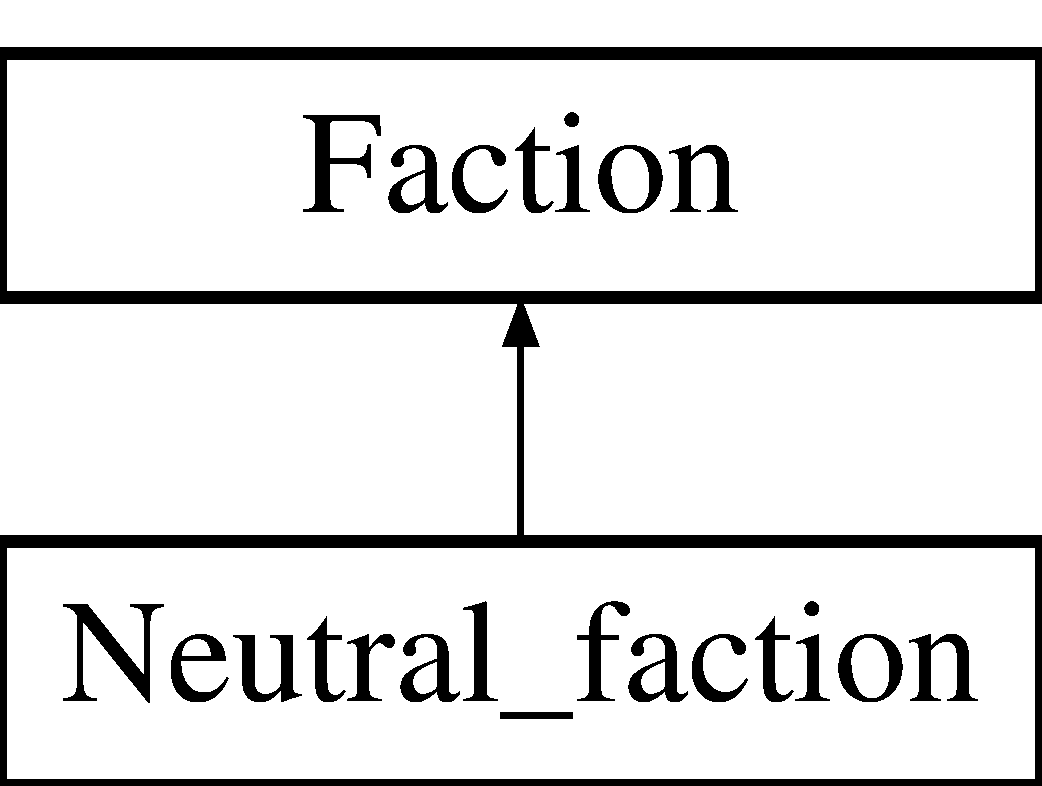
\includegraphics[height=2.000000cm]{classFaction}
\end{center}
\end{figure}
\subsection*{Fonctions membres publiques}
\begin{DoxyCompactItemize}
\item 
\hyperlink{classFaction_a470f14f0b1d94261d427a4673fe92421}{Faction} (\hyperlink{classWorld}{World} \&world, std\-::string name=\char`\"{}default\char`\"{}, Mother\-\_\-land $\ast$=nullptr)
\begin{DoxyCompactList}\small\item\em Constructeur. \end{DoxyCompactList}\item 
\hypertarget{classFaction_add5275f09ab0dd9a43dc7aa6e04e6e8a}{\hyperlink{classFaction}{Faction} \& \hyperlink{classFaction_add5275f09ab0dd9a43dc7aa6e04e6e8a}{operator=} (\hyperlink{classFaction}{Faction})}\label{classFaction_add5275f09ab0dd9a43dc7aa6e04e6e8a}

\begin{DoxyCompactList}\small\item\em Opérateur d'affectation, sans effet. \end{DoxyCompactList}\item 
\hypertarget{classFaction_a92285ba431e78a6fccb7ef1a9283dd65}{bool \hyperlink{classFaction_a92285ba431e78a6fccb7ef1a9283dd65}{operator==} (const \hyperlink{classFaction}{Faction} \&other) const }\label{classFaction_a92285ba431e78a6fccb7ef1a9283dd65}

\begin{DoxyCompactList}\small\item\em Comparateur avec une autre faction. \end{DoxyCompactList}\item 
\hypertarget{classFaction_adce9c9ccf9fe8a20a2680dd918a59a28}{bool \hyperlink{classFaction_adce9c9ccf9fe8a20a2680dd918a59a28}{operator==} (\hyperlink{classFaction}{Faction} \&other)}\label{classFaction_adce9c9ccf9fe8a20a2680dd918a59a28}

\begin{DoxyCompactList}\small\item\em Comparateur avec une autre faction. \end{DoxyCompactList}\item 
\hyperlink{classFaction}{Faction} $\ast$ \hyperlink{classFaction_aa398dcd8f3ca6cf694f69c2de152c538}{run} ()
\begin{DoxyCompactList}\small\item\em Lance le jeu. \end{DoxyCompactList}\item 
void \hyperlink{classFaction_a4f7c37fe385ee3a41e875aa23b6a8319}{init} ()
\begin{DoxyCompactList}\small\item\em Initialise la faction. \end{DoxyCompactList}\item 
void \hyperlink{classFaction_a144860993dcfd384b23da00219ed0b88}{die} ()
\begin{DoxyCompactList}\small\item\em Tue la faction. \end{DoxyCompactList}\item 
\hypertarget{classFaction_ac8ff16ef1f7fa6ba418ae7cf37406170}{std\-::string \hyperlink{classFaction_ac8ff16ef1f7fa6ba418ae7cf37406170}{get\-\_\-name} ()}\label{classFaction_ac8ff16ef1f7fa6ba418ae7cf37406170}

\begin{DoxyCompactList}\small\item\em Nom de la colonie. \end{DoxyCompactList}\item 
\hypertarget{classFaction_a0630bba70db7fc1881a5d0a2c7cac1c6}{double \hyperlink{classFaction_a0630bba70db7fc1881a5d0a2c7cac1c6}{get\-\_\-money} ()}\label{classFaction_a0630bba70db7fc1881a5d0a2c7cac1c6}

\begin{DoxyCompactList}\small\item\em Argent disponible. \end{DoxyCompactList}\item 
\hypertarget{classFaction_ad533ba9bbe8db562be988889553daf14}{char \hyperlink{classFaction_ad533ba9bbe8db562be988889553daf14}{get\-\_\-motherland\-\_\-symbol} ()}\label{classFaction_ad533ba9bbe8db562be988889553daf14}

\begin{DoxyCompactList}\small\item\em Caractère représentant la planète mère. \end{DoxyCompactList}\item 
\hypertarget{classFaction_a72aec7ed1856741ef6ec6cec3049c057}{char \hyperlink{classFaction_a72aec7ed1856741ef6ec6cec3049c057}{get\-\_\-colony\-\_\-symbol} ()}\label{classFaction_a72aec7ed1856741ef6ec6cec3049c057}

\begin{DoxyCompactList}\small\item\em Caractère représentant une colonie. \end{DoxyCompactList}\item 
\hypertarget{classFaction_a2e31e6fb93e25c7bac4a7e3d28ac4169}{std\-::string \hyperlink{classFaction_a2e31e6fb93e25c7bac4a7e3d28ac4169}{get\-\_\-colony\-\_\-color\-\_\-name} ()}\label{classFaction_a2e31e6fb93e25c7bac4a7e3d28ac4169}

\begin{DoxyCompactList}\small\item\em Couleur x11 des colonies. \end{DoxyCompactList}\item 
\hypertarget{classFaction_a4258c106abb09cb851a21980b8fc4996}{std\-::string \hyperlink{classFaction_a4258c106abb09cb851a21980b8fc4996}{get\-\_\-motherland\-\_\-color\-\_\-name} ()}\label{classFaction_a4258c106abb09cb851a21980b8fc4996}

\begin{DoxyCompactList}\small\item\em Couleur x11 de la planète mère. \end{DoxyCompactList}\item 
\hypertarget{classFaction_a4e27a1269e4e34e6abfed1302a9cf7e3}{\hyperlink{classMother__land}{Mother\-\_\-land} $\ast$ \hyperlink{classFaction_a4e27a1269e4e34e6abfed1302a9cf7e3}{get\-\_\-motherland\-\_\-} ()}\label{classFaction_a4e27a1269e4e34e6abfed1302a9cf7e3}

\begin{DoxyCompactList}\small\item\em Planète mère. \end{DoxyCompactList}\item 
\hypertarget{classFaction_a54e816116f2274310608bd6dfcf65dad}{std\-::list$<$ \hyperlink{classColonized__planet}{Colonized\-\_\-planet} $\ast$ $>$ \& \hyperlink{classFaction_a54e816116f2274310608bd6dfcf65dad}{get\-\_\-colonies} ()}\label{classFaction_a54e816116f2274310608bd6dfcf65dad}

\begin{DoxyCompactList}\small\item\em Liste des colonies. \end{DoxyCompactList}\item 
\hypertarget{classFaction_ab5d7a35b69eab9770069c27f2b61d527}{void \hyperlink{classFaction_ab5d7a35b69eab9770069c27f2b61d527}{add\-\_\-colony} (\hyperlink{classColonized__planet}{Colonized\-\_\-planet} $\ast$colony)}\label{classFaction_ab5d7a35b69eab9770069c27f2b61d527}

\begin{DoxyCompactList}\small\item\em Ajoute une colonie à la faction. \end{DoxyCompactList}\item 
void \hyperlink{classFaction_a0806d816ec82da48403a87a515e9ad0a}{remove\-\_\-colony} (\hyperlink{classColonized__planet}{Colonized\-\_\-planet} $\ast$colony)
\begin{DoxyCompactList}\small\item\em Supprime une colonie. \end{DoxyCompactList}\item 
void \hyperlink{classFaction_a5c704bccee1f3c845b3b521429bc4e60}{remove\-\_\-mother\-\_\-land} ()
\begin{DoxyCompactList}\small\item\em Supprime la planète mère. \end{DoxyCompactList}\item 
void \hyperlink{classFaction_ae90c4eab208071323dbc6c0991a22051}{remove\-\_\-demand} (\hyperlink{classColonized__planet}{Colonized\-\_\-planet} $\ast$colony)
\begin{DoxyCompactList}\small\item\em Supprime une demande de fonds. \end{DoxyCompactList}\item 
void \hyperlink{classFaction_ab550ddb4adcb6d480e4004915e7f20ce}{add\-\_\-to\-\_\-banque} (double)
\begin{DoxyCompactList}\small\item\em Ajoute de l'argent généré à la banque. \end{DoxyCompactList}\item 
\hypertarget{classFaction_a07b25ba27c0c8d158cb2310d064cc8a4}{void \hyperlink{classFaction_a07b25ba27c0c8d158cb2310d064cc8a4}{set\-\_\-colony\-\_\-symbol} (char c)}\label{classFaction_a07b25ba27c0c8d158cb2310d064cc8a4}

\begin{DoxyCompactList}\small\item\em Définit le caractère représentant une colonie. \end{DoxyCompactList}\item 
\hypertarget{classFaction_a9c1d1b8ab782174bf113ad7183cfe0c3}{void \hyperlink{classFaction_a9c1d1b8ab782174bf113ad7183cfe0c3}{set\-\_\-motherland\-\_\-symbol} (char c)}\label{classFaction_a9c1d1b8ab782174bf113ad7183cfe0c3}

\begin{DoxyCompactList}\small\item\em Définit le caractère représentant la planète mère. \end{DoxyCompactList}\item 
\hypertarget{classFaction_a51eadaa457179270f1950ed84e44df56}{void \hyperlink{classFaction_a51eadaa457179270f1950ed84e44df56}{set\-\_\-colony\-\_\-color\-\_\-name} (std\-::string colony\-\_\-color\-\_\-name)}\label{classFaction_a51eadaa457179270f1950ed84e44df56}

\begin{DoxyCompactList}\small\item\em Définit la couleur des colonies. \end{DoxyCompactList}\item 
\hypertarget{classFaction_ab17a2eabec14355868177554502972c7}{void \hyperlink{classFaction_ab17a2eabec14355868177554502972c7}{set\-\_\-motherland\-\_\-color\-\_\-name} (std\-::string motherland\-\_\-color\-\_\-name)}\label{classFaction_ab17a2eabec14355868177554502972c7}

\begin{DoxyCompactList}\small\item\em Définit la couleur de la planète mère. \end{DoxyCompactList}\item 
void \hyperlink{classFaction_a8a61c34f87a1d1f1284aba39c4887595}{add\-\_\-demand} (\hyperlink{classColonized__planet}{Colonized\-\_\-planet} $\ast$, double)
\begin{DoxyCompactList}\small\item\em Ajoute une demande de fonds à la liste des demandes. \end{DoxyCompactList}\item 
\hypertarget{classFaction_ac9c04d847c334eb3b5dc8a8dbe61586d}{double \hyperlink{classFaction_ac9c04d847c334eb3b5dc8a8dbe61586d}{get\-\_\-money\-\_\-spent} ()}\label{classFaction_ac9c04d847c334eb3b5dc8a8dbe61586d}

\begin{DoxyCompactList}\small\item\em Argent dépensé \end{DoxyCompactList}\item 
\hypertarget{classFaction_ada676ea8a06f80c2710adf1243d48db2}{double \hyperlink{classFaction_ada676ea8a06f80c2710adf1243d48db2}{get\-\_\-money\-\_\-produce\-\_\-} ()}\label{classFaction_ada676ea8a06f80c2710adf1243d48db2}

\begin{DoxyCompactList}\small\item\em Argent généré \end{DoxyCompactList}\item 
\hypertarget{classFaction_a7b174edbce20f49b7331665cb589e2f3}{int \hyperlink{classFaction_a7b174edbce20f49b7331665cb589e2f3}{get\-\_\-nb\-\_\-successful\-\_\-attack\-\_\-} ()}\label{classFaction_a7b174edbce20f49b7331665cb589e2f3}

\begin{DoxyCompactList}\small\item\em Attaques réussies. \end{DoxyCompactList}\item 
\hypertarget{classFaction_a70bbfa3dc7d4bf441d98984814f9abd1}{int \hyperlink{classFaction_a70bbfa3dc7d4bf441d98984814f9abd1}{get\-\_\-nb\-\_\-failed\-\_\-attack\-\_\-} ()}\label{classFaction_a70bbfa3dc7d4bf441d98984814f9abd1}

\begin{DoxyCompactList}\small\item\em Attaques échouées. \end{DoxyCompactList}\item 
\hypertarget{classFaction_a3d92bdbf463e4bd24824d058d58966f4}{void \hyperlink{classFaction_a3d92bdbf463e4bd24824d058d58966f4}{inc\-\_\-nb\-\_\-successful\-\_\-attack\-\_\-} ()}\label{classFaction_a3d92bdbf463e4bd24824d058d58966f4}

\begin{DoxyCompactList}\small\item\em Augmente le compteur d'attaques réussies. \end{DoxyCompactList}\item 
\hypertarget{classFaction_a29fcb8a676a70b4d0981546bf928bf73}{void \hyperlink{classFaction_a29fcb8a676a70b4d0981546bf928bf73}{inc\-\_\-nb\-\_\-failed\-\_\-attack\-\_\-} ()}\label{classFaction_a29fcb8a676a70b4d0981546bf928bf73}

\begin{DoxyCompactList}\small\item\em Augmente le compteur d'attaques échouées. \end{DoxyCompactList}\item 
std\-::string \hyperlink{classFaction_a75e7b414c89b8a4d75bf4a778e844b74}{to\-String} ()
\begin{DoxyCompactList}\small\item\em Texte représentant une faction. \end{DoxyCompactList}\end{DoxyCompactItemize}
\subsection*{Attributs privés}
\begin{DoxyCompactItemize}
\item 
\hypertarget{classFaction_a6d79b916267324627cddbfc04a4c9a64}{\hyperlink{classWorld}{World} \& \hyperlink{classFaction_a6d79b916267324627cddbfc04a4c9a64}{world\-\_\-}}\label{classFaction_a6d79b916267324627cddbfc04a4c9a64}

\begin{DoxyCompactList}\small\item\em Monde auquel est rattachée la faction. \end{DoxyCompactList}\item 
\hypertarget{classFaction_a632028ec500010c59419327a4cce3532}{std\-::string \hyperlink{classFaction_a632028ec500010c59419327a4cce3532}{name\-\_\-}}\label{classFaction_a632028ec500010c59419327a4cce3532}

\begin{DoxyCompactList}\small\item\em Nom de la faction. \end{DoxyCompactList}\item 
\hypertarget{classFaction_a7414f60b810c31e115e8f6995d47aa6e}{double \hyperlink{classFaction_a7414f60b810c31e115e8f6995d47aa6e}{money\-\_\-}}\label{classFaction_a7414f60b810c31e115e8f6995d47aa6e}

\begin{DoxyCompactList}\small\item\em Argent possédé par la faction. \end{DoxyCompactList}\item 
\hypertarget{classFaction_af9ece6405c2dc01b16a18be59ff2893e}{\hyperlink{classMother__land}{Mother\-\_\-land} $\ast$ \hyperlink{classFaction_af9ece6405c2dc01b16a18be59ff2893e}{motherland\-\_\-}}\label{classFaction_af9ece6405c2dc01b16a18be59ff2893e}

\begin{DoxyCompactList}\small\item\em Planète qui gère la faction. \end{DoxyCompactList}\item 
\hypertarget{classFaction_aee4de39f54f688641def6c0af48dfb29}{char \hyperlink{classFaction_aee4de39f54f688641def6c0af48dfb29}{motherland\-\_\-symbol\-\_\-}}\label{classFaction_aee4de39f54f688641def6c0af48dfb29}

\begin{DoxyCompactList}\small\item\em Caractère représentant la planète mère. \end{DoxyCompactList}\item 
\hypertarget{classFaction_af79e92739f25528585a539cefd719169}{std\-::list$<$ \hyperlink{classColonized__planet}{Colonized\-\_\-planet} $\ast$ $>$ \hyperlink{classFaction_af79e92739f25528585a539cefd719169}{colonies\-\_\-}}\label{classFaction_af79e92739f25528585a539cefd719169}

\begin{DoxyCompactList}\small\item\em Liste des colonies de la faction. \end{DoxyCompactList}\item 
\hypertarget{classFaction_a3c87e113f23c7638ec3ae447076f9f4a}{char \hyperlink{classFaction_a3c87e113f23c7638ec3ae447076f9f4a}{colony\-\_\-symbol\-\_\-}}\label{classFaction_a3c87e113f23c7638ec3ae447076f9f4a}

\begin{DoxyCompactList}\small\item\em Caractère représentant les colonies. \end{DoxyCompactList}\item 
\hypertarget{classFaction_aff4c256d6a30079ab09d5a9507003440}{std\-::string \hyperlink{classFaction_aff4c256d6a30079ab09d5a9507003440}{colony\-\_\-color\-\_\-name\-\_\-}}\label{classFaction_aff4c256d6a30079ab09d5a9507003440}

\begin{DoxyCompactList}\small\item\em Nom de la couleur représentant la colonie (x11names) \end{DoxyCompactList}\item 
\hypertarget{classFaction_ac67cd3b073d08e8dc3ac91a52a9daac0}{std\-::string \hyperlink{classFaction_ac67cd3b073d08e8dc3ac91a52a9daac0}{motherland\-\_\-color\-\_\-name\-\_\-}}\label{classFaction_ac67cd3b073d08e8dc3ac91a52a9daac0}

\begin{DoxyCompactList}\small\item\em Nom de la couleur représentant la planète mère (x11names) \end{DoxyCompactList}\item 
\hypertarget{classFaction_a6b7e2884e11b6c194e3399a318fda710}{std\-::list$<$ std\-::pair\\*
$<$ \hyperlink{classColonized__planet}{Colonized\-\_\-planet} $\ast$, double $>$ $>$ \hyperlink{classFaction_a6b7e2884e11b6c194e3399a318fda710}{demands\-\_\-}}\label{classFaction_a6b7e2884e11b6c194e3399a318fda710}

\begin{DoxyCompactList}\small\item\em Liste des demandes de fonds associées à la planète demandeuse. \end{DoxyCompactList}\item 
\hypertarget{classFaction_ab2bf963b863c933fc8ed642fb40e5a2d}{double \hyperlink{classFaction_ab2bf963b863c933fc8ed642fb40e5a2d}{money\-\_\-spent\-\_\-}}\label{classFaction_ab2bf963b863c933fc8ed642fb40e5a2d}

\begin{DoxyCompactList}\small\item\em Argent dépensé \end{DoxyCompactList}\item 
\hypertarget{classFaction_a36bb2676770658222036e8a946d12970}{double \hyperlink{classFaction_a36bb2676770658222036e8a946d12970}{money\-\_\-produce\-\_\-}}\label{classFaction_a36bb2676770658222036e8a946d12970}

\begin{DoxyCompactList}\small\item\em Argent généré \end{DoxyCompactList}\item 
\hypertarget{classFaction_a8638c6f131570f20510d6430df54500e}{int \hyperlink{classFaction_a8638c6f131570f20510d6430df54500e}{nb\-\_\-successful\-\_\-attack\-\_\-}}\label{classFaction_a8638c6f131570f20510d6430df54500e}

\begin{DoxyCompactList}\small\item\em Attaques réussies. \end{DoxyCompactList}\item 
\hypertarget{classFaction_a95acbb795c24778afabd22df2a6fb12e}{int \hyperlink{classFaction_a95acbb795c24778afabd22df2a6fb12e}{nb\-\_\-failed\-\_\-attack\-\_\-}}\label{classFaction_a95acbb795c24778afabd22df2a6fb12e}

\begin{DoxyCompactList}\small\item\em Attaques échouées. \end{DoxyCompactList}\end{DoxyCompactItemize}


\subsection{Description détaillée}
Entité de jeu, ensemble de planètes. 

Une faction est un groupement de colonies. Une faction est dirigée par une planète mère.

\begin{DoxyNote}{Note}
La mort de la planète mère induit la mort de la faction. 
\end{DoxyNote}


\subsection{Documentation des constructeurs et destructeur}
\hypertarget{classFaction_a470f14f0b1d94261d427a4673fe92421}{\index{Faction@{Faction}!Faction@{Faction}}
\index{Faction@{Faction}!Faction@{Faction}}
\subsubsection[{Faction}]{\setlength{\rightskip}{0pt plus 5cm}Faction\-::\-Faction (
\begin{DoxyParamCaption}
\item[{{\bf World} \&}]{world, }
\item[{std\-::string}]{name = {\ttfamily \char`\"{}default\char`\"{}}, }
\item[{{\bf Mother\-\_\-land} $\ast$}]{mother\-\_\-land = {\ttfamily nullptr}}
\end{DoxyParamCaption}
)}}\label{classFaction_a470f14f0b1d94261d427a4673fe92421}


Constructeur. 


\begin{DoxyParams}{Paramètres}
{\em world} & Monde auquel appartient la faction \\
\hline
{\em name} & Nom de la faction \\
\hline
{\em mother\-\_\-land} & Planète mère de la faction \\
\hline
\end{DoxyParams}


\subsection{Documentation des fonctions membres}
\hypertarget{classFaction_a8a61c34f87a1d1f1284aba39c4887595}{\index{Faction@{Faction}!add\-\_\-demand@{add\-\_\-demand}}
\index{add\-\_\-demand@{add\-\_\-demand}!Faction@{Faction}}
\subsubsection[{add\-\_\-demand}]{\setlength{\rightskip}{0pt plus 5cm}void Faction\-::add\-\_\-demand (
\begin{DoxyParamCaption}
\item[{{\bf Colonized\-\_\-planet} $\ast$}]{demander, }
\item[{double}]{cost}
\end{DoxyParamCaption}
)}}\label{classFaction_a8a61c34f87a1d1f1284aba39c4887595}


Ajoute une demande de fonds à la liste des demandes. 


\begin{DoxyParams}{Paramètres}
{\em demander} & La planète effectuant la demande \\
\hline
{\em cost} & Le montant demandé \\
\hline
\end{DoxyParams}
\hypertarget{classFaction_ab550ddb4adcb6d480e4004915e7f20ce}{\index{Faction@{Faction}!add\-\_\-to\-\_\-banque@{add\-\_\-to\-\_\-banque}}
\index{add\-\_\-to\-\_\-banque@{add\-\_\-to\-\_\-banque}!Faction@{Faction}}
\subsubsection[{add\-\_\-to\-\_\-banque}]{\setlength{\rightskip}{0pt plus 5cm}void Faction\-::add\-\_\-to\-\_\-banque (
\begin{DoxyParamCaption}
\item[{double}]{adding\-\_\-money}
\end{DoxyParamCaption}
)}}\label{classFaction_ab550ddb4adcb6d480e4004915e7f20ce}


Ajoute de l'argent généré à la banque. 


\begin{DoxyParams}{Paramètres}
{\em adding\-\_\-money} & quantité d'argent à ajouter \\
\hline
\end{DoxyParams}
\hypertarget{classFaction_a144860993dcfd384b23da00219ed0b88}{\index{Faction@{Faction}!die@{die}}
\index{die@{die}!Faction@{Faction}}
\subsubsection[{die}]{\setlength{\rightskip}{0pt plus 5cm}void Faction\-::die (
\begin{DoxyParamCaption}
{}
\end{DoxyParamCaption}
)}}\label{classFaction_a144860993dcfd384b23da00219ed0b88}


Tue la faction. 

\begin{DoxyWarning}{Avertissement}
Provoque la suppression définitive des colonies 
\end{DoxyWarning}
\begin{DoxyNote}{Note}
Le voisinage et l'ordonnanceur sont mis à jour 
\end{DoxyNote}
\hypertarget{classFaction_a4f7c37fe385ee3a41e875aa23b6a8319}{\index{Faction@{Faction}!init@{init}}
\index{init@{init}!Faction@{Faction}}
\subsubsection[{init}]{\setlength{\rightskip}{0pt plus 5cm}void Faction\-::init (
\begin{DoxyParamCaption}
{}
\end{DoxyParamCaption}
)}}\label{classFaction_a4f7c37fe385ee3a41e875aa23b6a8319}


Initialise la faction. 

\begin{DoxyNote}{Note}
Crée la planète mère n'importe où sur la grille
\end{DoxyNote}
\begin{DoxyRefDesc}{A faire}
\item[\hyperlink{todo__todo000004}{A faire}]Vérifier si la place n'est pas déja occupée par une autre planète mère \end{DoxyRefDesc}
\hypertarget{classFaction_a0806d816ec82da48403a87a515e9ad0a}{\index{Faction@{Faction}!remove\-\_\-colony@{remove\-\_\-colony}}
\index{remove\-\_\-colony@{remove\-\_\-colony}!Faction@{Faction}}
\subsubsection[{remove\-\_\-colony}]{\setlength{\rightskip}{0pt plus 5cm}void Faction\-::remove\-\_\-colony (
\begin{DoxyParamCaption}
\item[{{\bf Colonized\-\_\-planet} $\ast$}]{colony}
\end{DoxyParamCaption}
)}}\label{classFaction_a0806d816ec82da48403a87a515e9ad0a}


Supprime une colonie. 


\begin{DoxyParams}{Paramètres}
{\em colony} & colonie à supprimer \\
\hline
\end{DoxyParams}
\hypertarget{classFaction_ae90c4eab208071323dbc6c0991a22051}{\index{Faction@{Faction}!remove\-\_\-demand@{remove\-\_\-demand}}
\index{remove\-\_\-demand@{remove\-\_\-demand}!Faction@{Faction}}
\subsubsection[{remove\-\_\-demand}]{\setlength{\rightskip}{0pt plus 5cm}void Faction\-::remove\-\_\-demand (
\begin{DoxyParamCaption}
\item[{{\bf Colonized\-\_\-planet} $\ast$}]{colony}
\end{DoxyParamCaption}
)}}\label{classFaction_ae90c4eab208071323dbc6c0991a22051}


Supprime une demande de fonds. 


\begin{DoxyParams}{Paramètres}
{\em colony} & colonie qui a initié la demande \\
\hline
\end{DoxyParams}
\hypertarget{classFaction_a5c704bccee1f3c845b3b521429bc4e60}{\index{Faction@{Faction}!remove\-\_\-mother\-\_\-land@{remove\-\_\-mother\-\_\-land}}
\index{remove\-\_\-mother\-\_\-land@{remove\-\_\-mother\-\_\-land}!Faction@{Faction}}
\subsubsection[{remove\-\_\-mother\-\_\-land}]{\setlength{\rightskip}{0pt plus 5cm}void Faction\-::remove\-\_\-mother\-\_\-land (
\begin{DoxyParamCaption}
{}
\end{DoxyParamCaption}
)}}\label{classFaction_a5c704bccee1f3c845b3b521429bc4e60}


Supprime la planète mère. 

\begin{DoxyNote}{Note}
Cette méthode ne détruit pas la faction. 
\end{DoxyNote}
\hypertarget{classFaction_aa398dcd8f3ca6cf694f69c2de152c538}{\index{Faction@{Faction}!run@{run}}
\index{run@{run}!Faction@{Faction}}
\subsubsection[{run}]{\setlength{\rightskip}{0pt plus 5cm}{\bf Faction} $\ast$ Faction\-::run (
\begin{DoxyParamCaption}
{}
\end{DoxyParamCaption}
)}}\label{classFaction_aa398dcd8f3ca6cf694f69c2de152c538}


Lance le jeu. 

Si la planète mère a été détruite, la faction est supprimée.

\begin{DoxySeeAlso}{Voir également}
\hyperlink{classFaction_a144860993dcfd384b23da00219ed0b88}{die()} 
\end{DoxySeeAlso}
\begin{DoxyReturn}{Renvoie}
pointeur sur la faction qui a été détruite. 
\end{DoxyReturn}
\begin{DoxyNote}{Note}
En cas de non-\/destruction de la faction, le pointeur est nul. 
\end{DoxyNote}
\hypertarget{classFaction_a75e7b414c89b8a4d75bf4a778e844b74}{\index{Faction@{Faction}!to\-String@{to\-String}}
\index{to\-String@{to\-String}!Faction@{Faction}}
\subsubsection[{to\-String}]{\setlength{\rightskip}{0pt plus 5cm}string Faction\-::to\-String (
\begin{DoxyParamCaption}
{}
\end{DoxyParamCaption}
)}}\label{classFaction_a75e7b414c89b8a4d75bf4a778e844b74}


Texte représentant une faction. 

\begin{DoxyReturn}{Renvoie}
bloc de texte reprenant les paramètres principaux et de statistiques 
\end{DoxyReturn}


La documentation de cette classe a été générée à partir des fichiers suivants \-:\begin{DoxyCompactItemize}
\item 
/home/pipissavy/\-Dropbox/\-Cours/\-I\-S\-I\-M\-A/\-Z\-Z2/simulation/simu\-\_\-multi\-\_\-agents/src/Faction.\-hpp\item 
/home/pipissavy/\-Dropbox/\-Cours/\-I\-S\-I\-M\-A/\-Z\-Z2/simulation/simu\-\_\-multi\-\_\-agents/src/Faction.\-cpp\end{DoxyCompactItemize}

\hypertarget{classFree__planet}{\section{Référence de la classe Free\-\_\-planet}
\label{classFree__planet}\index{Free\-\_\-planet@{Free\-\_\-planet}}
}


Planète libre.  




{\ttfamily \#include $<$Free\-\_\-planet.\-hpp$>$}

Graphe d'héritage de Free\-\_\-planet\-:\begin{figure}[H]
\begin{center}
\leavevmode
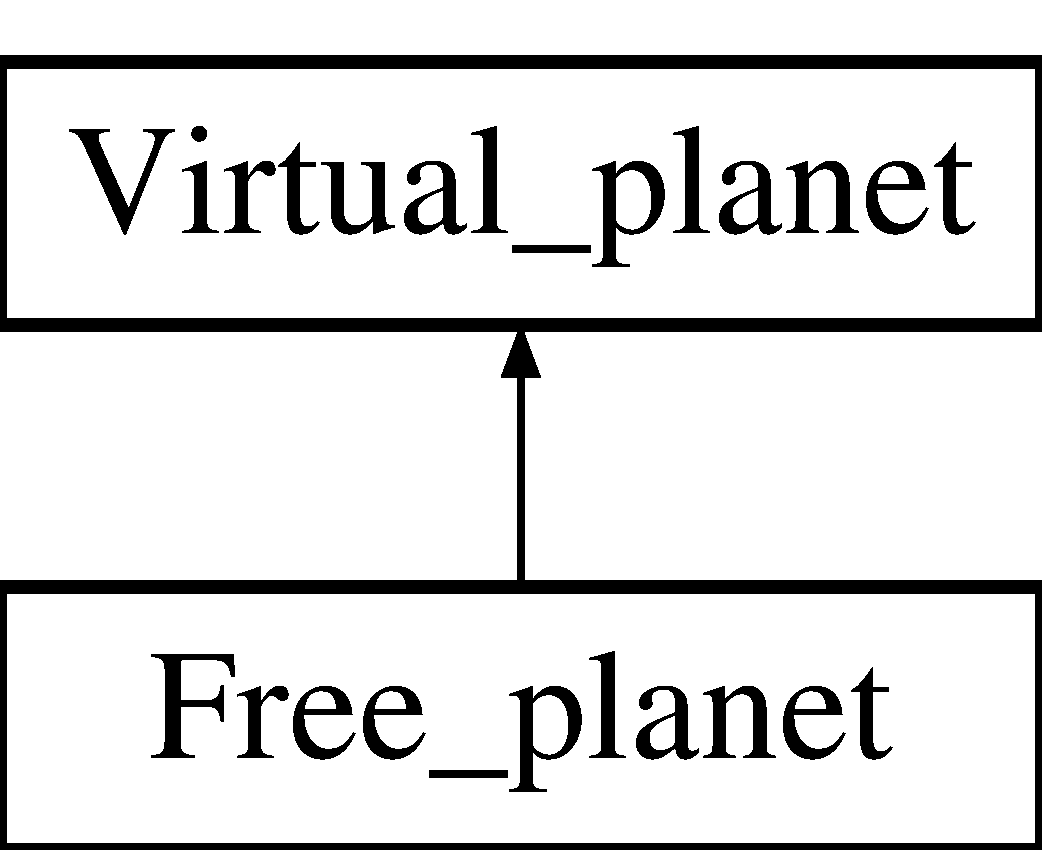
\includegraphics[height=2.000000cm]{classFree__planet}
\end{center}
\end{figure}
\subsection*{Fonctions membres publiques}
\begin{DoxyCompactItemize}
\item 
\hyperlink{classFree__planet_a7dfd0b5e9f41d84aba7ff721ec7a148e}{Free\-\_\-planet} (\hyperlink{classWorld}{World} \&, unsigned, unsigned)
\begin{DoxyCompactList}\small\item\em Constructeur. \end{DoxyCompactList}\item 
\hyperlink{classFree__planet_a40c231f6f967b35b0c13cb9f883bafe2}{Free\-\_\-planet} (\hyperlink{classColonized__planet}{Colonized\-\_\-planet} $\ast$)
\begin{DoxyCompactList}\small\item\em Crée une planète libre à partir d'une colonie. \end{DoxyCompactList}\item 
void \hyperlink{classFree__planet_a5ca63c483955025b2955eb35fea0f4e8}{run} ()
\begin{DoxyCompactList}\small\item\em Joue le tour. \end{DoxyCompactList}\item 
bool \hyperlink{classFree__planet_a205f5d75e430e9884b950b7bc1a3fe9d}{is\-\_\-attacked} (\hyperlink{classVirtual__planet}{Virtual\-\_\-planet} $\ast$)
\begin{DoxyCompactList}\small\item\em Répond à une attaque. \end{DoxyCompactList}\end{DoxyCompactItemize}
\subsection*{Membres hérités additionnels}


\subsection{Description détaillée}
Planète libre. 

Planète non encore colonisée. 

\subsection{Documentation des constructeurs et destructeur}
\hypertarget{classFree__planet_a7dfd0b5e9f41d84aba7ff721ec7a148e}{\index{Free\-\_\-planet@{Free\-\_\-planet}!Free\-\_\-planet@{Free\-\_\-planet}}
\index{Free\-\_\-planet@{Free\-\_\-planet}!Free_planet@{Free\-\_\-planet}}
\subsubsection[{Free\-\_\-planet}]{\setlength{\rightskip}{0pt plus 5cm}Free\-\_\-planet\-::\-Free\-\_\-planet (
\begin{DoxyParamCaption}
\item[{{\bf World} \&}]{world, }
\item[{unsigned}]{pos\-\_\-x, }
\item[{unsigned}]{pos\-\_\-y}
\end{DoxyParamCaption}
)}}\label{classFree__planet_a7dfd0b5e9f41d84aba7ff721ec7a148e}


Constructeur. 


\begin{DoxyParams}{Paramètres}
{\em world} & Monde auquel est rattachée la planète \\
\hline
{\em pos\-\_\-x} & Ligne sur la grille \\
\hline
{\em pos\-\_\-y} & Colonne sur la grille \\
\hline
\end{DoxyParams}
\hypertarget{classFree__planet_a40c231f6f967b35b0c13cb9f883bafe2}{\index{Free\-\_\-planet@{Free\-\_\-planet}!Free\-\_\-planet@{Free\-\_\-planet}}
\index{Free\-\_\-planet@{Free\-\_\-planet}!Free_planet@{Free\-\_\-planet}}
\subsubsection[{Free\-\_\-planet}]{\setlength{\rightskip}{0pt plus 5cm}Free\-\_\-planet\-::\-Free\-\_\-planet (
\begin{DoxyParamCaption}
\item[{{\bf Colonized\-\_\-planet} $\ast$}]{other}
\end{DoxyParamCaption}
)}}\label{classFree__planet_a40c231f6f967b35b0c13cb9f883bafe2}


Crée une planète libre à partir d'une colonie. 

\begin{DoxySeeAlso}{Voir également}
\hyperlink{classColonized__planet}{Colonized\-\_\-planet} 
\end{DoxySeeAlso}

\begin{DoxyParams}{Paramètres}
{\em other} & planète servant de base\\
\hline
\end{DoxyParams}
\begin{DoxyNote}{Note}
Met à jour le voisinage en remplaçant l'ancienne par la nouvelle planète. 
\end{DoxyNote}


\subsection{Documentation des fonctions membres}
\hypertarget{classFree__planet_a205f5d75e430e9884b950b7bc1a3fe9d}{\index{Free\-\_\-planet@{Free\-\_\-planet}!is\-\_\-attacked@{is\-\_\-attacked}}
\index{is\-\_\-attacked@{is\-\_\-attacked}!Free_planet@{Free\-\_\-planet}}
\subsubsection[{is\-\_\-attacked}]{\setlength{\rightskip}{0pt plus 5cm}bool Free\-\_\-planet\-::is\-\_\-attacked (
\begin{DoxyParamCaption}
\item[{{\bf Virtual\-\_\-planet} $\ast$}]{}
\end{DoxyParamCaption}
)\hspace{0.3cm}{\ttfamily [virtual]}}}\label{classFree__planet_a205f5d75e430e9884b950b7bc1a3fe9d}


Répond à une attaque. 

\begin{DoxyReturn}{Renvoie}
Booléen à vrai 4 fois sur 5 en moyenne 
\end{DoxyReturn}


Réimplémentée à partir de \hyperlink{classVirtual__planet_aa0712e85ae6ae7e9f05bd6d943a1a7b4}{Virtual\-\_\-planet}.

\hypertarget{classFree__planet_a5ca63c483955025b2955eb35fea0f4e8}{\index{Free\-\_\-planet@{Free\-\_\-planet}!run@{run}}
\index{run@{run}!Free_planet@{Free\-\_\-planet}}
\subsubsection[{run}]{\setlength{\rightskip}{0pt plus 5cm}void Free\-\_\-planet\-::run (
\begin{DoxyParamCaption}
{}
\end{DoxyParamCaption}
)}}\label{classFree__planet_a5ca63c483955025b2955eb35fea0f4e8}


Joue le tour. 

\begin{DoxyWarning}{Avertissement}
Ne doit jamais être appelée car une planète libre n'est pas sensée jouer. 
\end{DoxyWarning}


La documentation de cette classe a été générée à partir des fichiers suivants \-:\begin{DoxyCompactItemize}
\item 
/home/pipissavy/\-Dropbox/\-Cours/\-I\-S\-I\-M\-A/\-Z\-Z2/simulation/simu\-\_\-multi\-\_\-agents/src/Free\-\_\-planet.\-hpp\item 
/home/pipissavy/\-Dropbox/\-Cours/\-I\-S\-I\-M\-A/\-Z\-Z2/simulation/simu\-\_\-multi\-\_\-agents/src/Free\-\_\-planet.\-cpp\end{DoxyCompactItemize}

\hypertarget{classMainWindow}{\section{Référence de la classe Main\-Window}
\label{classMainWindow}\index{Main\-Window@{Main\-Window}}
}


Fenêtre principale.  




{\ttfamily \#include $<$mainwindow.\-h$>$}

Graphe d'héritage de Main\-Window\-:\begin{figure}[H]
\begin{center}
\leavevmode
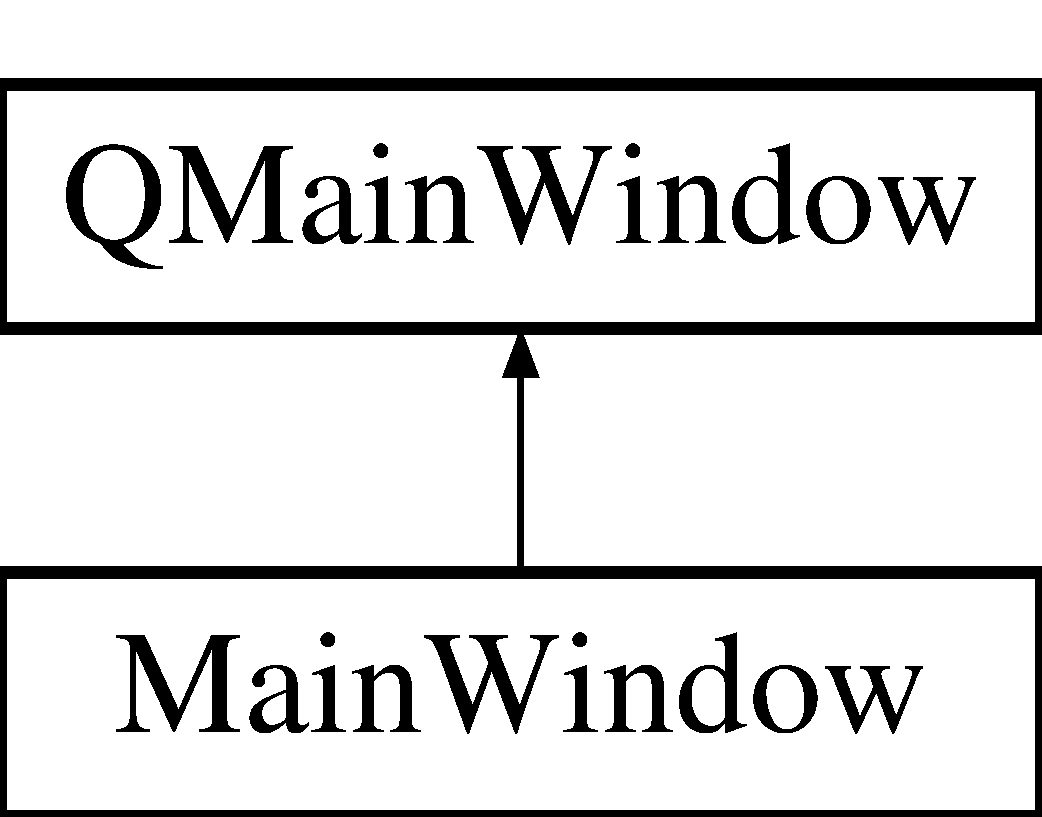
\includegraphics[height=2.000000cm]{classMainWindow}
\end{center}
\end{figure}
\subsection*{Fonctions membres publiques}
\begin{DoxyCompactItemize}
\item 
\hypertarget{classMainWindow_a8b244be8b7b7db1b08de2a2acb9409db}{{\bfseries Main\-Window} (Q\-Widget $\ast$parent=0)}\label{classMainWindow_a8b244be8b7b7db1b08de2a2acb9409db}

\item 
\hypertarget{classMainWindow_ae3d7a4598609a86e8bd317c0d85c4495}{void \hyperlink{classMainWindow_ae3d7a4598609a86e8bd317c0d85c4495}{show} ()}\label{classMainWindow_ae3d7a4598609a86e8bd317c0d85c4495}

\begin{DoxyCompactList}\small\item\em Affichage des objets contenus dans la fenêtre. \end{DoxyCompactList}\end{DoxyCompactItemize}
\subsection*{Attributs privés}
\begin{DoxyCompactItemize}
\item 
\hypertarget{classMainWindow_a35466a70ed47252a0191168126a352a5}{Ui\-::\-Main\-Window $\ast$ \hyperlink{classMainWindow_a35466a70ed47252a0191168126a352a5}{ui}}\label{classMainWindow_a35466a70ed47252a0191168126a352a5}

\begin{DoxyCompactList}\small\item\em Interface utilisateur, contient les différents objets et la structure. \end{DoxyCompactList}\end{DoxyCompactItemize}


\subsection{Description détaillée}
Fenêtre principale. 

La documentation de cette classe a été générée à partir des fichiers suivants \-:\begin{DoxyCompactItemize}
\item 
mainwindow.\-h\item 
mainwindow.\-cpp\end{DoxyCompactItemize}

\hypertarget{classMother__land}{\section{Référence de la classe Mother\-\_\-land}
\label{classMother__land}\index{Mother\-\_\-land@{Mother\-\_\-land}}
}


Planète mère.  




{\ttfamily \#include $<$Mother\-\_\-land.\-hpp$>$}

Graphe d'héritage de Mother\-\_\-land\-:\begin{figure}[H]
\begin{center}
\leavevmode
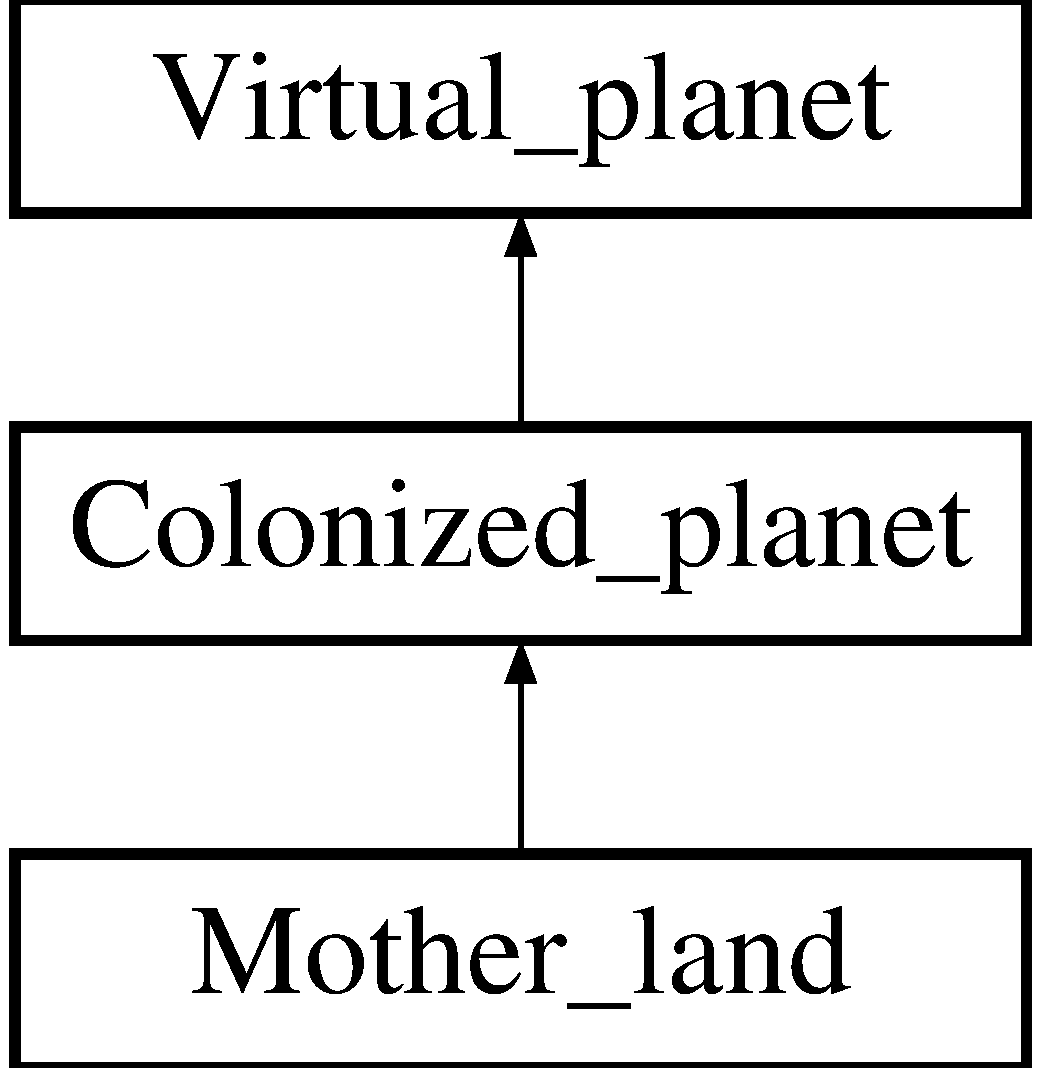
\includegraphics[height=3.000000cm]{classMother__land}
\end{center}
\end{figure}
\subsection*{Fonctions membres publiques}
\begin{DoxyCompactItemize}
\item 
\hyperlink{classMother__land_a8fd578b591a99a926bebd55959492997}{Mother\-\_\-land} (\hyperlink{classVirtual__planet}{Virtual\-\_\-planet} $\ast$, \hyperlink{classFaction}{Faction} \&)
\begin{DoxyCompactList}\small\item\em Constructeur. \end{DoxyCompactList}\item 
\hypertarget{classMother__land_ae50ab9634b50efcb8a9f0fe275342923}{char \hyperlink{classMother__land_ae50ab9634b50efcb8a9f0fe275342923}{display} ()}\label{classMother__land_ae50ab9634b50efcb8a9f0fe275342923}

\begin{DoxyCompactList}\small\item\em Caractère représentant la planète mère. \end{DoxyCompactList}\item 
\hypertarget{classMother__land_a2a862d8ca3bf717ef885edc50ea92a8d}{std\-::string \hyperlink{classMother__land_a2a862d8ca3bf717ef885edc50ea92a8d}{get\-\_\-color\-\_\-name} ()}\label{classMother__land_a2a862d8ca3bf717ef885edc50ea92a8d}

\begin{DoxyCompactList}\small\item\em Couleur représentant la planète mère. \end{DoxyCompactList}\item 
bool \hyperlink{classMother__land_a295325cdedbfcfb17c200a4a7438761c}{is\-\_\-attacked} (\hyperlink{classVirtual__planet}{Virtual\-\_\-planet} $\ast$)
\begin{DoxyCompactList}\small\item\em Répond à une attaque. \end{DoxyCompactList}\end{DoxyCompactItemize}
\subsection*{Membres hérités additionnels}


\subsection{Description détaillée}
Planète mère. 

Dirige une faction

\begin{DoxySeeAlso}{Voir également}
\hyperlink{classFaction}{Faction} 
\end{DoxySeeAlso}


\subsection{Documentation des constructeurs et destructeur}
\hypertarget{classMother__land_a8fd578b591a99a926bebd55959492997}{\index{Mother\-\_\-land@{Mother\-\_\-land}!Mother\-\_\-land@{Mother\-\_\-land}}
\index{Mother\-\_\-land@{Mother\-\_\-land}!Mother_land@{Mother\-\_\-land}}
\subsubsection[{Mother\-\_\-land}]{\setlength{\rightskip}{0pt plus 5cm}Mother\-\_\-land\-::\-Mother\-\_\-land (
\begin{DoxyParamCaption}
\item[{{\bf Virtual\-\_\-planet} $\ast$}]{fp, }
\item[{{\bf Faction} \&}]{fac}
\end{DoxyParamCaption}
)}}\label{classMother__land_a8fd578b591a99a926bebd55959492997}


Constructeur. 

Appelle le constructeur de \hyperlink{classColonized__planet}{Colonized\-\_\-planet}

\begin{DoxySeeAlso}{Voir également}
\hyperlink{classColonized__planet}{Colonized\-\_\-planet}
\end{DoxySeeAlso}

\begin{DoxyParams}{Paramètres}
{\em fp} & Planète présente précédemment \\
\hline
{\em fac} & \hyperlink{classFaction}{Faction} à laquelle est rattachée la planète mère \\
\hline
\end{DoxyParams}


\subsection{Documentation des fonctions membres}
\hypertarget{classMother__land_a295325cdedbfcfb17c200a4a7438761c}{\index{Mother\-\_\-land@{Mother\-\_\-land}!is\-\_\-attacked@{is\-\_\-attacked}}
\index{is\-\_\-attacked@{is\-\_\-attacked}!Mother_land@{Mother\-\_\-land}}
\subsubsection[{is\-\_\-attacked}]{\setlength{\rightskip}{0pt plus 5cm}bool Mother\-\_\-land\-::is\-\_\-attacked (
\begin{DoxyParamCaption}
\item[{{\bf Virtual\-\_\-planet} $\ast$}]{attacker}
\end{DoxyParamCaption}
)\hspace{0.3cm}{\ttfamily [virtual]}}}\label{classMother__land_a295325cdedbfcfb17c200a4a7438761c}


Répond à une attaque. 


\begin{DoxyParams}{Paramètres}
{\em attacker} & Planète attaquante \\
\hline
\end{DoxyParams}
\begin{DoxyReturn}{Renvoie}
vrai si l'attaquant n'appartient pas à la même faction
\end{DoxyReturn}
\begin{DoxyNote}{Note}
Tir ami interdit 
\end{DoxyNote}


Réimplémentée à partir de \hyperlink{classColonized__planet_af637772fb84e45bb47447c88aa8d3f4a}{Colonized\-\_\-planet}.



La documentation de cette classe a été générée à partir des fichiers suivants \-:\begin{DoxyCompactItemize}
\item 
/home/pipissavy/\-Dropbox/\-Cours/\-I\-S\-I\-M\-A/\-Z\-Z2/simulation/simu\-\_\-multi\-\_\-agents/src/Mother\-\_\-land.\-hpp\item 
/home/pipissavy/\-Dropbox/\-Cours/\-I\-S\-I\-M\-A/\-Z\-Z2/simulation/simu\-\_\-multi\-\_\-agents/src/Mother\-\_\-land.\-cpp\end{DoxyCompactItemize}

\hypertarget{classNeutral__faction}{\section{Référence de la classe Neutral\-\_\-faction}
\label{classNeutral__faction}\index{Neutral\-\_\-faction@{Neutral\-\_\-faction}}
}


\hyperlink{classFaction}{Faction} neutre.  




{\ttfamily \#include $<$Neutral\-\_\-faction.\-hpp$>$}

Graphe d'héritage de Neutral\-\_\-faction\-:\begin{figure}[H]
\begin{center}
\leavevmode
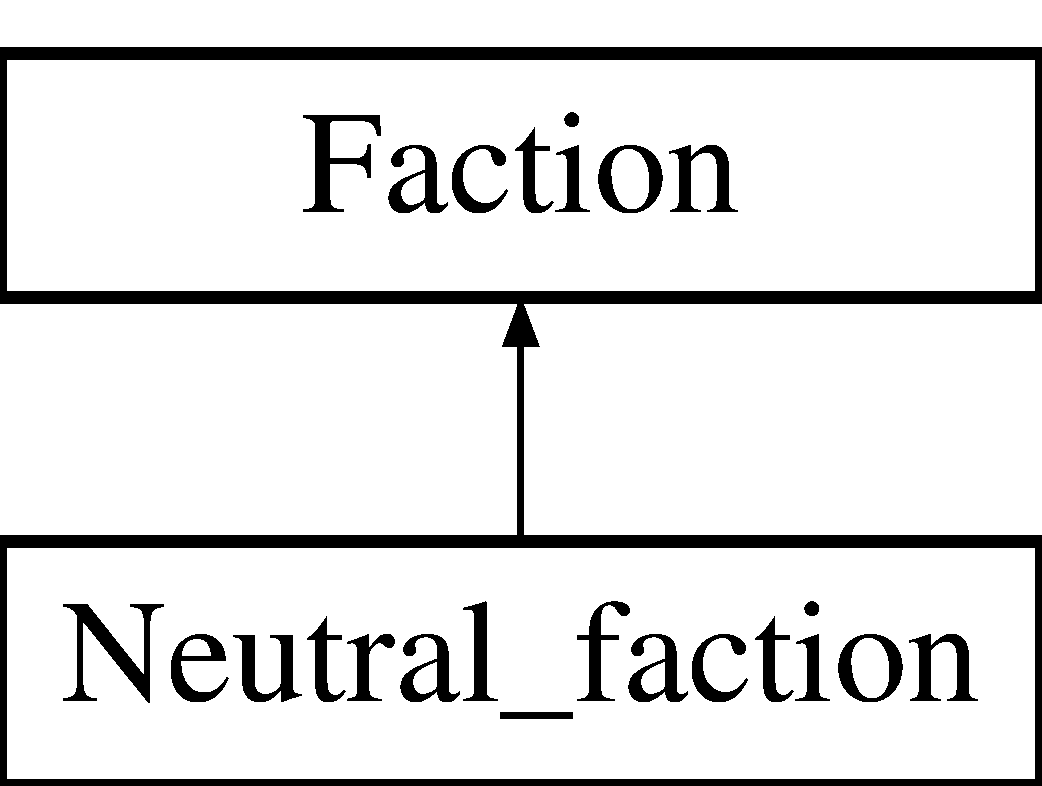
\includegraphics[height=2.000000cm]{classNeutral__faction}
\end{center}
\end{figure}
\subsection*{Fonctions membres publiques statiques}
\begin{DoxyCompactItemize}
\item 
static \hyperlink{classNeutral__faction}{Neutral\-\_\-faction} $\ast$ \hyperlink{classNeutral__faction_ae8e449bd58cfac78bc8cac249c7d1352}{get\-\_\-instance} (\hyperlink{classWorld}{World} \&world)
\begin{DoxyCompactList}\small\item\em Demande de la planète neutre. \end{DoxyCompactList}\item 
\hypertarget{classNeutral__faction_a1b42cda1fbc38de7408963f63e494d97}{static void \hyperlink{classNeutral__faction_a1b42cda1fbc38de7408963f63e494d97}{dispose} ()}\label{classNeutral__faction_a1b42cda1fbc38de7408963f63e494d97}

\begin{DoxyCompactList}\small\item\em Libère l'instance. \end{DoxyCompactList}\end{DoxyCompactItemize}
\subsection*{Fonctions membres privées}
\begin{DoxyCompactItemize}
\item 
\hyperlink{classNeutral__faction_aacd2a58a4ba2b640bac83a730bfaeeec}{Neutral\-\_\-faction} (\hyperlink{classWorld}{World} \&world)
\begin{DoxyCompactList}\small\item\em Constructeur. \end{DoxyCompactList}\end{DoxyCompactItemize}
\subsection*{Attributs privés statiques}
\begin{DoxyCompactItemize}
\item 
\hypertarget{classNeutral__faction_acf5e8d031f701352fb71a65568e9eb77}{static \hyperlink{classNeutral__faction}{Neutral\-\_\-faction} $\ast$ \hyperlink{classNeutral__faction_acf5e8d031f701352fb71a65568e9eb77}{instance\-\_\-} = nullptr}\label{classNeutral__faction_acf5e8d031f701352fb71a65568e9eb77}

\begin{DoxyCompactList}\small\item\em Instance (unique) \end{DoxyCompactList}\end{DoxyCompactItemize}
\subsection*{Membres hérités additionnels}


\subsection{Description détaillée}
\hyperlink{classFaction}{Faction} neutre. 

C'est la faction à laquelle appartiennent les planètes libres

\begin{DoxyNote}{Note}
Modèle singleton 
\end{DoxyNote}
\begin{DoxyRefDesc}{A faire}
\item[\hyperlink{todo__todo000005}{A faire}]à vérifier \end{DoxyRefDesc}


\subsection{Documentation des constructeurs et destructeur}
\hypertarget{classNeutral__faction_aacd2a58a4ba2b640bac83a730bfaeeec}{\index{Neutral\-\_\-faction@{Neutral\-\_\-faction}!Neutral\-\_\-faction@{Neutral\-\_\-faction}}
\index{Neutral\-\_\-faction@{Neutral\-\_\-faction}!Neutral_faction@{Neutral\-\_\-faction}}
\subsubsection[{Neutral\-\_\-faction}]{\setlength{\rightskip}{0pt plus 5cm}Neutral\-\_\-faction\-::\-Neutral\-\_\-faction (
\begin{DoxyParamCaption}
\item[{{\bf World} \&}]{world}
\end{DoxyParamCaption}
)\hspace{0.3cm}{\ttfamily [private]}}}\label{classNeutral__faction_aacd2a58a4ba2b640bac83a730bfaeeec}


Constructeur. 


\begin{DoxyParams}{Paramètres}
{\em world} & Monde auquel appartient la faction neutre \\
\hline
\end{DoxyParams}


\subsection{Documentation des fonctions membres}
\hypertarget{classNeutral__faction_ae8e449bd58cfac78bc8cac249c7d1352}{\index{Neutral\-\_\-faction@{Neutral\-\_\-faction}!get\-\_\-instance@{get\-\_\-instance}}
\index{get\-\_\-instance@{get\-\_\-instance}!Neutral_faction@{Neutral\-\_\-faction}}
\subsubsection[{get\-\_\-instance}]{\setlength{\rightskip}{0pt plus 5cm}{\bf Neutral\-\_\-faction} $\ast$ Neutral\-\_\-faction\-::get\-\_\-instance (
\begin{DoxyParamCaption}
\item[{{\bf World} \&}]{world}
\end{DoxyParamCaption}
)\hspace{0.3cm}{\ttfamily [static]}}}\label{classNeutral__faction_ae8e449bd58cfac78bc8cac249c7d1352}


Demande de la planète neutre. 


\begin{DoxyParams}{Paramètres}
{\em world} & Monde auquel la faction neutre appartient \\
\hline
\end{DoxyParams}
\begin{DoxyReturn}{Renvoie}
pointeur sur l'instance unique de la faction neutre 
\end{DoxyReturn}


La documentation de cette classe a été générée à partir des fichiers suivants \-:\begin{DoxyCompactItemize}
\item 
/home/pipissavy/\-Dropbox/\-Cours/\-I\-S\-I\-M\-A/\-Z\-Z2/simulation/simu\-\_\-multi\-\_\-agents/src/Neutral\-\_\-faction.\-hpp\item 
/home/pipissavy/\-Dropbox/\-Cours/\-I\-S\-I\-M\-A/\-Z\-Z2/simulation/simu\-\_\-multi\-\_\-agents/src/Neutral\-\_\-faction.\-cpp\end{DoxyCompactItemize}

\hypertarget{classVirtual__planet}{\section{Référence de la classe Virtual\-\_\-planet}
\label{classVirtual__planet}\index{Virtual\-\_\-planet@{Virtual\-\_\-planet}}
}


Planète virtuelle.  




{\ttfamily \#include $<$Virtual\-\_\-planet.\-hpp$>$}

Graphe d'héritage de Virtual\-\_\-planet\-:\begin{figure}[H]
\begin{center}
\leavevmode
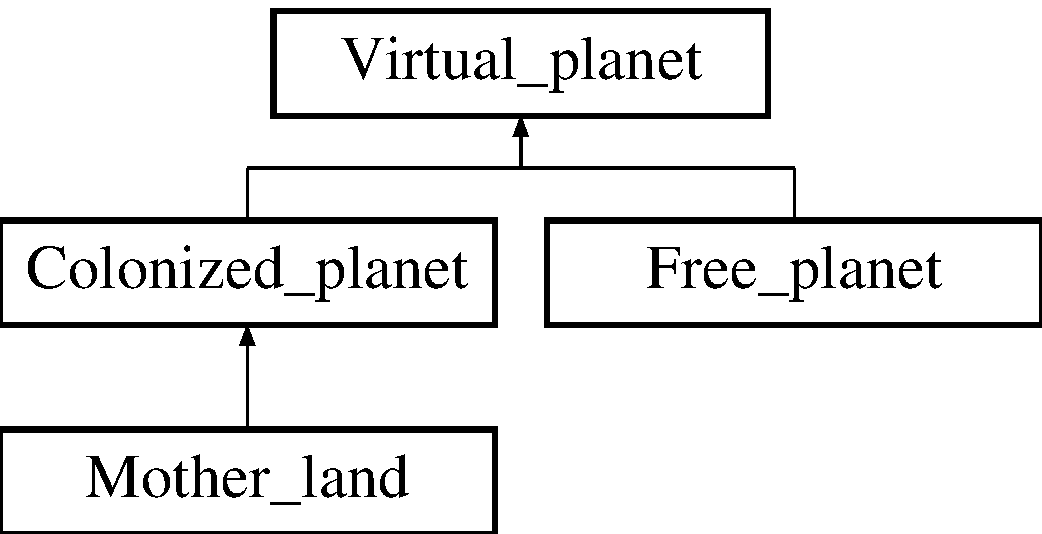
\includegraphics[height=3.000000cm]{classVirtual__planet}
\end{center}
\end{figure}
\subsection*{Fonctions membres publiques}
\begin{DoxyCompactItemize}
\item 
\hyperlink{classVirtual__planet_a16cc8781ce4c81e6365d87b659e5108c}{Virtual\-\_\-planet} (\hyperlink{classWorld}{World} \&, unsigned, unsigned)
\begin{DoxyCompactList}\small\item\em Constructeur. \end{DoxyCompactList}\item 
\hyperlink{classVirtual__planet_a4a2c71c2400d55bf861bc5d433123ac6}{Virtual\-\_\-planet} (\hyperlink{classVirtual__planet}{Virtual\-\_\-planet} $\ast$)
\begin{DoxyCompactList}\small\item\em Constructeur par copie. \end{DoxyCompactList}\item 
\hypertarget{classVirtual__planet_a029ab1668b417b73c57fae8dae82cc1c}{virtual \hyperlink{classVirtual__planet_a029ab1668b417b73c57fae8dae82cc1c}{$\sim$\-Virtual\-\_\-planet} ()}\label{classVirtual__planet_a029ab1668b417b73c57fae8dae82cc1c}

\begin{DoxyCompactList}\small\item\em Destructeur à redéfinir. \end{DoxyCompactList}\item 
\hypertarget{classVirtual__planet_aa17b2d88853c46485a3907f08148ef1e}{void \hyperlink{classVirtual__planet_aa17b2d88853c46485a3907f08148ef1e}{set\-\_\-neighbourhood} ()}\label{classVirtual__planet_aa17b2d88853c46485a3907f08148ef1e}

\begin{DoxyCompactList}\small\item\em Calcule le voisinage de la planète. \end{DoxyCompactList}\item 
void \hyperlink{classVirtual__planet_ae32d3dd758346701d6f8c6f6f8a46925}{set\-\_\-neighbourhood2} ()
\begin{DoxyCompactList}\small\item\em Calcule le voisinage de la planète. \end{DoxyCompactList}\item 
virtual void \hyperlink{classVirtual__planet_ac67c164e630df471819336d2404a99af}{update\-\_\-neighbourhood} (\hyperlink{classVirtual__planet}{Virtual\-\_\-planet} $\ast$, \hyperlink{classVirtual__planet}{Virtual\-\_\-planet} $\ast$)
\begin{DoxyCompactList}\small\item\em Met à jour le voisinage. \end{DoxyCompactList}\item 
\hypertarget{classVirtual__planet_aa0712e85ae6ae7e9f05bd6d943a1a7b4}{virtual bool \hyperlink{classVirtual__planet_aa0712e85ae6ae7e9f05bd6d943a1a7b4}{is\-\_\-attacked} (\hyperlink{classVirtual__planet}{Virtual\-\_\-planet} $\ast$)}\label{classVirtual__planet_aa0712e85ae6ae7e9f05bd6d943a1a7b4}

\begin{DoxyCompactList}\small\item\em Réponse lorsqu'une attaque est subie (vrai par défaut) \end{DoxyCompactList}\item 
void \hyperlink{classVirtual__planet_aa063b164739842ba1c95018e24b122d5}{run} ()
\begin{DoxyCompactList}\small\item\em Joue sur le plateau. \end{DoxyCompactList}\item 
\hypertarget{classVirtual__planet_a3294db05abde3781e5ed0625d5e094a6}{virtual void \hyperlink{classVirtual__planet_a3294db05abde3781e5ed0625d5e094a6}{reinitialisate\-\_\-target} ()}\label{classVirtual__planet_a3294db05abde3781e5ed0625d5e094a6}

\begin{DoxyCompactList}\small\item\em Réinitialisation de la cible, à redéfinir. \end{DoxyCompactList}\item 
bool \hyperlink{classVirtual__planet_ab47d3e56b68242189b6df870d45c5157}{has\-\_\-changed} ()
\begin{DoxyCompactList}\small\item\em Récupère un changement. \end{DoxyCompactList}\item 
\hypertarget{classVirtual__planet_a21eeef694b6dc66b7a394bda53e9c360}{virtual bool \hyperlink{classVirtual__planet_a21eeef694b6dc66b7a394bda53e9c360}{can\-\_\-be\-\_\-replaced} ()}\label{classVirtual__planet_a21eeef694b6dc66b7a394bda53e9c360}

\begin{DoxyCompactList}\small\item\em Renvoie true si la planete n'est pas un agent. \end{DoxyCompactList}\item 
\hypertarget{classVirtual__planet_affaf5157ca3fb7e3d5c9fac1736578a3}{virtual char \hyperlink{classVirtual__planet_affaf5157ca3fb7e3d5c9fac1736578a3}{display} ()}\label{classVirtual__planet_affaf5157ca3fb7e3d5c9fac1736578a3}

\begin{DoxyCompactList}\small\item\em Caractère par défaut (point) \end{DoxyCompactList}\item 
\hypertarget{classVirtual__planet_a7f442fee301927b27217877abb765833}{virtual double \hyperlink{classVirtual__planet_a7f442fee301927b27217877abb765833}{estimate\-\_\-cost} ()}\label{classVirtual__planet_a7f442fee301927b27217877abb765833}

\begin{DoxyCompactList}\small\item\em Estime le cout d'une attaque. \end{DoxyCompactList}\item 
\hypertarget{classVirtual__planet_a84cba41f0fa06d0512ea462a26b972e3}{virtual std\-::string \hyperlink{classVirtual__planet_a84cba41f0fa06d0512ea462a26b972e3}{get\-\_\-color\-\_\-name} ()}\label{classVirtual__planet_a84cba41f0fa06d0512ea462a26b972e3}

\begin{DoxyCompactList}\small\item\em Couleur par défaut (gris) \end{DoxyCompactList}\item 
virtual \hyperlink{classFaction}{Faction} \& \hyperlink{classVirtual__planet_ac0d0e30029566b9113652c04ec2e6599}{get\-\_\-faction} ()
\begin{DoxyCompactList}\small\item\em Obtenir la faction à laquelle appartient la planète. \end{DoxyCompactList}\item 
\hypertarget{classVirtual__planet_acccedbd81a89f4ad75a6a5c1c09b044c}{virtual unsigned \hyperlink{classVirtual__planet_acccedbd81a89f4ad75a6a5c1c09b044c}{pos\-\_\-x} ()}\label{classVirtual__planet_acccedbd81a89f4ad75a6a5c1c09b044c}

\begin{DoxyCompactList}\small\item\em Ligne dans la grille. \end{DoxyCompactList}\item 
\hypertarget{classVirtual__planet_a3453bf12cb4d348aee6594c127ba6a56}{virtual unsigned \hyperlink{classVirtual__planet_a3453bf12cb4d348aee6594c127ba6a56}{pos\-\_\-y} ()}\label{classVirtual__planet_a3453bf12cb4d348aee6594c127ba6a56}

\begin{DoxyCompactList}\small\item\em Colonne dans la grille. \end{DoxyCompactList}\item 
\hypertarget{classVirtual__planet_a1d3474a2ca3833a770c3763884a84323}{\hyperlink{classWorld}{World} \& \hyperlink{classVirtual__planet_a1d3474a2ca3833a770c3763884a84323}{get\-\_\-world} ()}\label{classVirtual__planet_a1d3474a2ca3833a770c3763884a84323}

\begin{DoxyCompactList}\small\item\em Monde auquel appartient la planète. \end{DoxyCompactList}\item 
\hypertarget{classVirtual__planet_a25045d61c5ee29b94de56db88fa96f98}{virtual double \hyperlink{classVirtual__planet_a25045d61c5ee29b94de56db88fa96f98}{get\-\_\-defense} ()}\label{classVirtual__planet_a25045d61c5ee29b94de56db88fa96f98}

\begin{DoxyCompactList}\small\item\em Défense de base. \end{DoxyCompactList}\item 
\hypertarget{classVirtual__planet_a4294d3312671d720dca0b72a1648e6a4}{virtual double \hyperlink{classVirtual__planet_a4294d3312671d720dca0b72a1648e6a4}{get\-\_\-production} ()}\label{classVirtual__planet_a4294d3312671d720dca0b72a1648e6a4}

\begin{DoxyCompactList}\small\item\em Productivité de base. \end{DoxyCompactList}\item 
\hypertarget{classVirtual__planet_a996699dcad7e99262842e06079896ed1}{std\-::vector$<$ \hyperlink{classVirtual__planet}{Virtual\-\_\-planet} $\ast$ $>$ \hyperlink{classVirtual__planet_a996699dcad7e99262842e06079896ed1}{get\-\_\-neighbourhood} ()}\label{classVirtual__planet_a996699dcad7e99262842e06079896ed1}

\begin{DoxyCompactList}\small\item\em Liste des voisins. \end{DoxyCompactList}\end{DoxyCompactItemize}
\subsection*{Fonctions membres protégées}
\begin{DoxyCompactItemize}
\item 
\hypertarget{classVirtual__planet_a9c79d42a13bb25243354faf9895aca14}{void \hyperlink{classVirtual__planet_a9c79d42a13bb25243354faf9895aca14}{change} ()}\label{classVirtual__planet_a9c79d42a13bb25243354faf9895aca14}

\begin{DoxyCompactList}\small\item\em Signale un changement d'état. \end{DoxyCompactList}\end{DoxyCompactItemize}
\subsection*{Attributs protégés}
\begin{DoxyCompactItemize}
\item 
\hypertarget{classVirtual__planet_a16ff82fac346eec9d2229fb8c09e3807}{\hyperlink{classWorld}{World} \& \hyperlink{classVirtual__planet_a16ff82fac346eec9d2229fb8c09e3807}{world\-\_\-}}\label{classVirtual__planet_a16ff82fac346eec9d2229fb8c09e3807}

\begin{DoxyCompactList}\small\item\em Monde auquel appartient la planète. \end{DoxyCompactList}\item 
\hypertarget{classVirtual__planet_ad03593bd1a1236933b638f6079f639b1}{unsigned \hyperlink{classVirtual__planet_ad03593bd1a1236933b638f6079f639b1}{pos\-\_\-x\-\_\-}}\label{classVirtual__planet_ad03593bd1a1236933b638f6079f639b1}

\begin{DoxyCompactList}\small\item\em Ligne dans la grille. \end{DoxyCompactList}\item 
\hypertarget{classVirtual__planet_aa7e03c8010b64d2528d5edb5651962a9}{unsigned \hyperlink{classVirtual__planet_aa7e03c8010b64d2528d5edb5651962a9}{pos\-\_\-y\-\_\-}}\label{classVirtual__planet_aa7e03c8010b64d2528d5edb5651962a9}

\begin{DoxyCompactList}\small\item\em Colonne dans la grille. \end{DoxyCompactList}\item 
\hypertarget{classVirtual__planet_a353b64093f5c146de64a2f694738b65b}{std\-::vector$<$ \hyperlink{classVirtual__planet}{Virtual\-\_\-planet} $\ast$ $>$ \hyperlink{classVirtual__planet_a353b64093f5c146de64a2f694738b65b}{neighbourhood\-\_\-}}\label{classVirtual__planet_a353b64093f5c146de64a2f694738b65b}

\begin{DoxyCompactList}\small\item\em Liste des voisins. \end{DoxyCompactList}\item 
\hypertarget{classVirtual__planet_aa5ebb40e5a4ed0a631b120749f938f35}{bool \hyperlink{classVirtual__planet_aa5ebb40e5a4ed0a631b120749f938f35}{changed\-\_\-}}\label{classVirtual__planet_aa5ebb40e5a4ed0a631b120749f938f35}

\begin{DoxyCompactList}\small\item\em Etat changé \end{DoxyCompactList}\item 
double \hyperlink{classVirtual__planet_a6f8de6a5104185b9c36c64a45260fab6}{production\-\_\-rate\-\_\-}
\begin{DoxyCompactList}\small\item\em Taux de production entre M\-I\-N\-\_\-\-P\-R\-O\-D\-U\-C\-T\-I\-O\-N\-\_\-\-R\-A\-T\-E et M\-A\-X\-\_\-\-P\-R\-O\-D\-U\-C\-T\-I\-O\-N\-\_\-\-R\-A\-T\-E. \end{DoxyCompactList}\item 
double \hyperlink{classVirtual__planet_af62ede97e609fd17818af229799dbe3b}{natural\-\_\-defense\-\_\-}
\begin{DoxyCompactList}\small\item\em Taux de défense naturelle entre M\-I\-N\-\_\-\-N\-A\-T\-U\-R\-A\-L\-\_\-\-D\-E\-F\-E\-N\-S\-E et M\-A\-X\-\_\-\-N\-A\-T\-U\-R\-A\-L\-\_\-\-D\-E\-F\-E\-N\-S\-E. \end{DoxyCompactList}\end{DoxyCompactItemize}
\subsection*{Attributs protégés statiques}
\begin{DoxyCompactItemize}
\item 
\hypertarget{classVirtual__planet_a5c08ee009e9d9d0b284b133e18c2b7f9}{static const int \hyperlink{classVirtual__planet_a5c08ee009e9d9d0b284b133e18c2b7f9}{M\-I\-N\-\_\-\-P\-R\-O\-D\-U\-C\-T\-I\-O\-N\-\_\-\-R\-A\-T\-E} = 0}\label{classVirtual__planet_a5c08ee009e9d9d0b284b133e18c2b7f9}

\begin{DoxyCompactList}\small\item\em Taux de production minimal. \end{DoxyCompactList}\item 
\hypertarget{classVirtual__planet_a0899115c7ae16c4e07e6319209b678cc}{static const int \hyperlink{classVirtual__planet_a0899115c7ae16c4e07e6319209b678cc}{M\-A\-X\-\_\-\-P\-R\-O\-D\-U\-C\-T\-I\-O\-N\-\_\-\-R\-A\-T\-E} = 15}\label{classVirtual__planet_a0899115c7ae16c4e07e6319209b678cc}

\begin{DoxyCompactList}\small\item\em Taux de production maximal. \end{DoxyCompactList}\item 
\hypertarget{classVirtual__planet_ae0e71188803de0af557c7a1db8bd2d95}{static const int \hyperlink{classVirtual__planet_ae0e71188803de0af557c7a1db8bd2d95}{M\-I\-N\-\_\-\-N\-A\-T\-U\-R\-A\-L\-\_\-\-D\-E\-F\-E\-N\-S\-E} = 25}\label{classVirtual__planet_ae0e71188803de0af557c7a1db8bd2d95}

\begin{DoxyCompactList}\small\item\em Taux de défense naturelle minimal. \end{DoxyCompactList}\item 
\hypertarget{classVirtual__planet_ad5b8a23606fded6c444a93136fceab0a}{static const int \hyperlink{classVirtual__planet_ad5b8a23606fded6c444a93136fceab0a}{M\-A\-X\-\_\-\-N\-A\-T\-U\-R\-A\-L\-\_\-\-D\-E\-F\-E\-N\-S\-E} = 50}\label{classVirtual__planet_ad5b8a23606fded6c444a93136fceab0a}

\begin{DoxyCompactList}\small\item\em Taux de défense naturelle maximal. \end{DoxyCompactList}\end{DoxyCompactItemize}


\subsection{Description détaillée}
Planète virtuelle. 

Planète servant de base à toutes les autres. Contient tous les paramètres communs 

\subsection{Documentation des constructeurs et destructeur}
\hypertarget{classVirtual__planet_a16cc8781ce4c81e6365d87b659e5108c}{\index{Virtual\-\_\-planet@{Virtual\-\_\-planet}!Virtual\-\_\-planet@{Virtual\-\_\-planet}}
\index{Virtual\-\_\-planet@{Virtual\-\_\-planet}!Virtual_planet@{Virtual\-\_\-planet}}
\subsubsection[{Virtual\-\_\-planet}]{\setlength{\rightskip}{0pt plus 5cm}Virtual\-\_\-planet\-::\-Virtual\-\_\-planet (
\begin{DoxyParamCaption}
\item[{{\bf World} \&}]{world, }
\item[{unsigned}]{pos\-\_\-x, }
\item[{unsigned}]{pos\-\_\-y}
\end{DoxyParamCaption}
)}}\label{classVirtual__planet_a16cc8781ce4c81e6365d87b659e5108c}


Constructeur. 


\begin{DoxyParams}{Paramètres}
{\em world} & Monde auquel la planète appartient \\
\hline
{\em pos\-\_\-x} & Ligne dans la grille \\
\hline
{\em pos\-\_\-y} & Colonne dans la grille \\
\hline
\end{DoxyParams}
\hypertarget{classVirtual__planet_a4a2c71c2400d55bf861bc5d433123ac6}{\index{Virtual\-\_\-planet@{Virtual\-\_\-planet}!Virtual\-\_\-planet@{Virtual\-\_\-planet}}
\index{Virtual\-\_\-planet@{Virtual\-\_\-planet}!Virtual_planet@{Virtual\-\_\-planet}}
\subsubsection[{Virtual\-\_\-planet}]{\setlength{\rightskip}{0pt plus 5cm}Virtual\-\_\-planet\-::\-Virtual\-\_\-planet (
\begin{DoxyParamCaption}
\item[{{\bf Virtual\-\_\-planet} $\ast$}]{other}
\end{DoxyParamCaption}
)}}\label{classVirtual__planet_a4a2c71c2400d55bf861bc5d433123ac6}


Constructeur par copie. 


\begin{DoxyParams}{Paramètres}
{\em other} & Planète d'origine \\
\hline
\end{DoxyParams}


\subsection{Documentation des fonctions membres}
\hypertarget{classVirtual__planet_ac0d0e30029566b9113652c04ec2e6599}{\index{Virtual\-\_\-planet@{Virtual\-\_\-planet}!get\-\_\-faction@{get\-\_\-faction}}
\index{get\-\_\-faction@{get\-\_\-faction}!Virtual_planet@{Virtual\-\_\-planet}}
\subsubsection[{get\-\_\-faction}]{\setlength{\rightskip}{0pt plus 5cm}{\bf Faction} \& Virtual\-\_\-planet\-::get\-\_\-faction (
\begin{DoxyParamCaption}
{}
\end{DoxyParamCaption}
)\hspace{0.3cm}{\ttfamily [virtual]}}}\label{classVirtual__planet_ac0d0e30029566b9113652c04ec2e6599}


Obtenir la faction à laquelle appartient la planète. 

\begin{DoxyReturn}{Renvoie}
\hyperlink{classFaction}{Faction} neutre par défaut 
\end{DoxyReturn}


Réimplémentée dans \hyperlink{classColonized__planet_a78748eadea1186e104ccc247a1d1f546}{Colonized\-\_\-planet}.

\hypertarget{classVirtual__planet_ab47d3e56b68242189b6df870d45c5157}{\index{Virtual\-\_\-planet@{Virtual\-\_\-planet}!has\-\_\-changed@{has\-\_\-changed}}
\index{has\-\_\-changed@{has\-\_\-changed}!Virtual_planet@{Virtual\-\_\-planet}}
\subsubsection[{has\-\_\-changed}]{\setlength{\rightskip}{0pt plus 5cm}bool Virtual\-\_\-planet\-::has\-\_\-changed (
\begin{DoxyParamCaption}
{}
\end{DoxyParamCaption}
)}}\label{classVirtual__planet_ab47d3e56b68242189b6df870d45c5157}


Récupère un changement. 

\begin{DoxyReturn}{Renvoie}
l'état de changement
\end{DoxyReturn}
\begin{DoxyNote}{Note}
réinitialise l'état de changement s'il était actif 
\end{DoxyNote}
\hypertarget{classVirtual__planet_aa063b164739842ba1c95018e24b122d5}{\index{Virtual\-\_\-planet@{Virtual\-\_\-planet}!run@{run}}
\index{run@{run}!Virtual_planet@{Virtual\-\_\-planet}}
\subsubsection[{run}]{\setlength{\rightskip}{0pt plus 5cm}void Virtual\-\_\-planet\-::run (
\begin{DoxyParamCaption}
{}
\end{DoxyParamCaption}
)}}\label{classVirtual__planet_aa063b164739842ba1c95018e24b122d5}


Joue sur le plateau. 

\begin{DoxyNote}{Note}
Non utilisée 
\end{DoxyNote}
\hypertarget{classVirtual__planet_ae32d3dd758346701d6f8c6f6f8a46925}{\index{Virtual\-\_\-planet@{Virtual\-\_\-planet}!set\-\_\-neighbourhood2@{set\-\_\-neighbourhood2}}
\index{set\-\_\-neighbourhood2@{set\-\_\-neighbourhood2}!Virtual_planet@{Virtual\-\_\-planet}}
\subsubsection[{set\-\_\-neighbourhood2}]{\setlength{\rightskip}{0pt plus 5cm}void Virtual\-\_\-planet\-::set\-\_\-neighbourhood2 (
\begin{DoxyParamCaption}
{}
\end{DoxyParamCaption}
)}}\label{classVirtual__planet_ae32d3dd758346701d6f8c6f6f8a46925}


Calcule le voisinage de la planète. 

\begin{DoxyNote}{Note}
Grille torique 
\end{DoxyNote}
\hypertarget{classVirtual__planet_ac67c164e630df471819336d2404a99af}{\index{Virtual\-\_\-planet@{Virtual\-\_\-planet}!update\-\_\-neighbourhood@{update\-\_\-neighbourhood}}
\index{update\-\_\-neighbourhood@{update\-\_\-neighbourhood}!Virtual_planet@{Virtual\-\_\-planet}}
\subsubsection[{update\-\_\-neighbourhood}]{\setlength{\rightskip}{0pt plus 5cm}void Virtual\-\_\-planet\-::update\-\_\-neighbourhood (
\begin{DoxyParamCaption}
\item[{{\bf Virtual\-\_\-planet} $\ast$}]{old\-\_\-one, }
\item[{{\bf Virtual\-\_\-planet} $\ast$}]{new\-\_\-one}
\end{DoxyParamCaption}
)\hspace{0.3cm}{\ttfamily [virtual]}}}\label{classVirtual__planet_ac67c164e630df471819336d2404a99af}


Met à jour le voisinage. 


\begin{DoxyParams}{Paramètres}
{\em old\-\_\-one} & planète à remplacer \\
\hline
{\em new\-\_\-one} & planète remplaçante \\
\hline
\end{DoxyParams}


Réimplémentée dans \hyperlink{classColonized__planet_ac4f99490dc15c7715c1b476a490228a4}{Colonized\-\_\-planet}.



\subsection{Documentation des données membres}
\hypertarget{classVirtual__planet_af62ede97e609fd17818af229799dbe3b}{\index{Virtual\-\_\-planet@{Virtual\-\_\-planet}!natural\-\_\-defense\-\_\-@{natural\-\_\-defense\-\_\-}}
\index{natural\-\_\-defense\-\_\-@{natural\-\_\-defense\-\_\-}!Virtual_planet@{Virtual\-\_\-planet}}
\subsubsection[{natural\-\_\-defense\-\_\-}]{\setlength{\rightskip}{0pt plus 5cm}double Virtual\-\_\-planet\-::natural\-\_\-defense\-\_\-\hspace{0.3cm}{\ttfamily [protected]}}}\label{classVirtual__planet_af62ede97e609fd17818af229799dbe3b}


Taux de défense naturelle entre M\-I\-N\-\_\-\-N\-A\-T\-U\-R\-A\-L\-\_\-\-D\-E\-F\-E\-N\-S\-E et M\-A\-X\-\_\-\-N\-A\-T\-U\-R\-A\-L\-\_\-\-D\-E\-F\-E\-N\-S\-E. 

\begin{DoxySeeAlso}{Voir également}
\hyperlink{classVirtual__planet_ae0e71188803de0af557c7a1db8bd2d95}{M\-I\-N\-\_\-\-N\-A\-T\-U\-R\-A\-L\-\_\-\-D\-E\-F\-E\-N\-S\-E} 

\hyperlink{classVirtual__planet_ad5b8a23606fded6c444a93136fceab0a}{M\-A\-X\-\_\-\-N\-A\-T\-U\-R\-A\-L\-\_\-\-D\-E\-F\-E\-N\-S\-E} 
\end{DoxySeeAlso}
\hypertarget{classVirtual__planet_a6f8de6a5104185b9c36c64a45260fab6}{\index{Virtual\-\_\-planet@{Virtual\-\_\-planet}!production\-\_\-rate\-\_\-@{production\-\_\-rate\-\_\-}}
\index{production\-\_\-rate\-\_\-@{production\-\_\-rate\-\_\-}!Virtual_planet@{Virtual\-\_\-planet}}
\subsubsection[{production\-\_\-rate\-\_\-}]{\setlength{\rightskip}{0pt plus 5cm}double Virtual\-\_\-planet\-::production\-\_\-rate\-\_\-\hspace{0.3cm}{\ttfamily [protected]}}}\label{classVirtual__planet_a6f8de6a5104185b9c36c64a45260fab6}


Taux de production entre M\-I\-N\-\_\-\-P\-R\-O\-D\-U\-C\-T\-I\-O\-N\-\_\-\-R\-A\-T\-E et M\-A\-X\-\_\-\-P\-R\-O\-D\-U\-C\-T\-I\-O\-N\-\_\-\-R\-A\-T\-E. 

\begin{DoxySeeAlso}{Voir également}
\hyperlink{classVirtual__planet_a5c08ee009e9d9d0b284b133e18c2b7f9}{M\-I\-N\-\_\-\-P\-R\-O\-D\-U\-C\-T\-I\-O\-N\-\_\-\-R\-A\-T\-E} 

\hyperlink{classVirtual__planet_a0899115c7ae16c4e07e6319209b678cc}{M\-A\-X\-\_\-\-P\-R\-O\-D\-U\-C\-T\-I\-O\-N\-\_\-\-R\-A\-T\-E} 
\end{DoxySeeAlso}


La documentation de cette classe a été générée à partir des fichiers suivants \-:\begin{DoxyCompactItemize}
\item 
/home/pipissavy/\-Dropbox/\-Cours/\-I\-S\-I\-M\-A/\-Z\-Z2/simulation/simu\-\_\-multi\-\_\-agents/src/Virtual\-\_\-planet.\-hpp\item 
/home/pipissavy/\-Dropbox/\-Cours/\-I\-S\-I\-M\-A/\-Z\-Z2/simulation/simu\-\_\-multi\-\_\-agents/src/Virtual\-\_\-planet.\-cpp\end{DoxyCompactItemize}

\hypertarget{classWorld}{\section{Référence de la classe World}
\label{classWorld}\index{World@{World}}
}


Monde du jeu, possédant la grille.  




{\ttfamily \#include $<$World.\-hpp$>$}

\subsection*{Fonctions membres publiques}
\begin{DoxyCompactItemize}
\item 
\hyperlink{classWorld_ac6dabb39d0af2594d84dde35ec79c585}{World} (unsigned \hyperlink{classWorld_a9263bc299d1446cc7435c58fc70dbc12}{len}=20, unsigned \hyperlink{classWorld_abb70914eb0c8c9a083372c679b512a84}{hei}=20)
\begin{DoxyCompactList}\small\item\em Constructeur. \end{DoxyCompactList}\item 
\hypertarget{classWorld_a8c73fba541a5817fff65147ba47cd827}{\hyperlink{classWorld_a8c73fba541a5817fff65147ba47cd827}{$\sim$\-World} ()}\label{classWorld_a8c73fba541a5817fff65147ba47cd827}

\begin{DoxyCompactList}\small\item\em Destructeur. \end{DoxyCompactList}\item 
time\-\_\-h \hyperlink{classWorld_a6d23268873d3e6dc117d6c76fc87626b}{start} ()
\begin{DoxyCompactList}\small\item\em Lance la simulation. \end{DoxyCompactList}\item 
void \hyperlink{classWorld_a26aa2658c22414b5f572df8cb5efbeae}{scheduler} ()
\begin{DoxyCompactList}\small\item\em Ordonnanceur. \end{DoxyCompactList}\item 
\hypertarget{classWorld_af50a03db2f7a2fea3a013557251d5a7c}{void \hyperlink{classWorld_af50a03db2f7a2fea3a013557251d5a7c}{test2factions} ()}\label{classWorld_af50a03db2f7a2fea3a013557251d5a7c}

\begin{DoxyCompactList}\small\item\em Exemple de simulation avec 2 factions. \end{DoxyCompactList}\item 
\hypertarget{classWorld_aeff7e2c21e886b7a7d5793354644858f}{void \hyperlink{classWorld_aeff7e2c21e886b7a7d5793354644858f}{test3factions} ()}\label{classWorld_aeff7e2c21e886b7a7d5793354644858f}

\begin{DoxyCompactList}\small\item\em Exemple de simulation avec 3 factions. \end{DoxyCompactList}\item 
\hypertarget{classWorld_ae093b6af05143a8faa53db9774eb77ff}{void \hyperlink{classWorld_ae093b6af05143a8faa53db9774eb77ff}{test4factions} ()}\label{classWorld_ae093b6af05143a8faa53db9774eb77ff}

\begin{DoxyCompactList}\small\item\em Exemple de simulation avec 4 factions. \end{DoxyCompactList}\item 
void \hyperlink{classWorld_a007f9908bb224a8fb4b6b58820971eed}{display} ()
\begin{DoxyCompactList}\small\item\em Affichage de la grille. \end{DoxyCompactList}\item 
void \hyperlink{classWorld_ab01f5891ce4a1532563b4674de788daf}{remove\-\_\-faction} (\hyperlink{classFaction}{Faction} $\ast$)
\begin{DoxyCompactList}\small\item\em Suppression définitive d'une faction. \end{DoxyCompactList}\item 
void \hyperlink{classWorld_adfedeb704ce247d881bd9565d9d867d4}{add\-\_\-waiting\-\_\-agent} (\hyperlink{classColonized__planet}{Colonized\-\_\-planet} $\ast$)
\begin{DoxyCompactList}\small\item\em Ajout d'un agent à la liste d'attente. \end{DoxyCompactList}\item 
void \hyperlink{classWorld_a5abd90500d2a6e70ef6d21dbc02cb440}{remove\-\_\-waiting\-\_\-agent} (\hyperlink{classColonized__planet}{Colonized\-\_\-planet} $\ast$)
\begin{DoxyCompactList}\small\item\em Suppression d'un agent de la liste d'attente. \end{DoxyCompactList}\item 
\hyperlink{classVirtual__planet}{Virtual\-\_\-planet} $\ast$ \hyperlink{classWorld_a6c5e27cae9fd6a526da0f4c58b320733}{get\-\_\-grid} (unsigned x, unsigned y)
\begin{DoxyCompactList}\small\item\em Planète dans la grille. \end{DoxyCompactList}\item 
void \hyperlink{classWorld_a593960e61c13083719721b0c289dad94}{set\-\_\-grid} (\hyperlink{classVirtual__planet}{Virtual\-\_\-planet} $\ast$, unsigned x, unsigned y)
\begin{DoxyCompactList}\small\item\em Installe une planète dans la grille. \end{DoxyCompactList}\item 
\hypertarget{classWorld_a9263bc299d1446cc7435c58fc70dbc12}{unsigned \hyperlink{classWorld_a9263bc299d1446cc7435c58fc70dbc12}{len} () const }\label{classWorld_a9263bc299d1446cc7435c58fc70dbc12}

\begin{DoxyCompactList}\small\item\em Nombre de places sur une ligne. \end{DoxyCompactList}\item 
\hypertarget{classWorld_abb70914eb0c8c9a083372c679b512a84}{unsigned \hyperlink{classWorld_abb70914eb0c8c9a083372c679b512a84}{hei} () const }\label{classWorld_abb70914eb0c8c9a083372c679b512a84}

\begin{DoxyCompactList}\small\item\em Nombre de places sur une colonne. \end{DoxyCompactList}\item 
\hypertarget{classWorld_ae8473fc069907cd6cc96d32c49b62d7e}{bool \hyperlink{classWorld_ae8473fc069907cd6cc96d32c49b62d7e}{is\-Ended} ()}\label{classWorld_ae8473fc069907cd6cc96d32c49b62d7e}

\begin{DoxyCompactList}\small\item\em Vrai si la partie est terminée. \end{DoxyCompactList}\item 
std\-::list$<$ \hyperlink{classFaction}{Faction} $>$ \hyperlink{classWorld_afcbc72644f2fc56f223c9bb80b50474a}{get\-\_\-factions} ()
\begin{DoxyCompactList}\small\item\em Liste des factions. \end{DoxyCompactList}\item 
string \hyperlink{classWorld_a2ae945389cb96c6a10dcc07a45a2cefd}{stats} ()
\begin{DoxyCompactList}\small\item\em Statistiques. \end{DoxyCompactList}\item 
string \hyperlink{classWorld_aaa59a538a6b688f164707743faf63072}{get\-\_\-winner\-\_\-name} ()
\begin{DoxyCompactList}\small\item\em Nom de la faction gagnante. \end{DoxyCompactList}\end{DoxyCompactItemize}
\subsection*{Fonctions membres publiques statiques}
\begin{DoxyCompactItemize}
\item 
static int \hyperlink{classWorld_ae1a517e48a53300f77b9715f2d05da9f}{gen\-\_\-mt} ()
\begin{DoxyCompactList}\small\item\em Générateur aléatoire (Mersenne Twister) \end{DoxyCompactList}\item 
static int \hyperlink{classWorld_a5e407254abb3e35217524fe37f8a6a82}{gen\-\_\-mt} (int a, int b)
\begin{DoxyCompactList}\small\item\em Générateur aléatoire borné par un intervalle. \end{DoxyCompactList}\item 
static int \hyperlink{classWorld_aeeb9732117c1ed11efd98d17b1177e54}{gen\-\_\-mt\-\_\-shuffle} (int i)
\begin{DoxyCompactList}\small\item\em Générateur aléatoire borné supérieurement. \end{DoxyCompactList}\item 
\hypertarget{classWorld_abf19b18c7eb174377bf99b41aa84e769}{static void \hyperlink{classWorld_abf19b18c7eb174377bf99b41aa84e769}{dispose} ()}\label{classWorld_abf19b18c7eb174377bf99b41aa84e769}

\begin{DoxyCompactList}\small\item\em Nettoie la faction neutre. \end{DoxyCompactList}\end{DoxyCompactItemize}
\subsection*{Attributs privés}
\begin{DoxyCompactItemize}
\item 
\hypertarget{classWorld_a5773dad1dda0f5380a5f65c94f57de9c}{bool \hyperlink{classWorld_a5773dad1dda0f5380a5f65c94f57de9c}{end\-\_\-}}\label{classWorld_a5773dad1dda0f5380a5f65c94f57de9c}

\begin{DoxyCompactList}\small\item\em Fin de la partie. \end{DoxyCompactList}\item 
\hypertarget{classWorld_a46afecbf41a86494f6e48dad3d4a3247}{std\-::vector$<$ std\-::vector\\*
$<$ \hyperlink{classVirtual__planet}{Virtual\-\_\-planet} $\ast$ $>$ $>$ \hyperlink{classWorld_a46afecbf41a86494f6e48dad3d4a3247}{grid\-\_\-}}\label{classWorld_a46afecbf41a86494f6e48dad3d4a3247}

\begin{DoxyCompactList}\small\item\em Grille de jeu. \end{DoxyCompactList}\item 
\hypertarget{classWorld_a9e4a76505c85cae1329f6083011e9be5}{std\-::list$<$ \hyperlink{classFaction}{Faction} $>$ \hyperlink{classWorld_a9e4a76505c85cae1329f6083011e9be5}{factions\-\_\-}}\label{classWorld_a9e4a76505c85cae1329f6083011e9be5}

\begin{DoxyCompactList}\small\item\em Liste des factions en jeu. \end{DoxyCompactList}\item 
std\-::vector$<$ \hyperlink{classColonized__planet}{Colonized\-\_\-planet} $\ast$ $>$ \hyperlink{classWorld_a732ce05c7e0012b98e2a8715b41d89fd}{waiting\-\_\-agents\-\_\-}
\begin{DoxyCompactList}\small\item\em Liste des agents n'ayant pas encore joué \end{DoxyCompactList}\item 
\hypertarget{classWorld_aafbe82365fac0f0d0e98c95d33a258f9}{std\-::vector$<$ \hyperlink{classColonized__planet}{Colonized\-\_\-planet} $\ast$ $>$ \hyperlink{classWorld_aafbe82365fac0f0d0e98c95d33a258f9}{already\-\_\-run\-\_\-agents\-\_\-}}\label{classWorld_aafbe82365fac0f0d0e98c95d33a258f9}

\begin{DoxyCompactList}\small\item\em Liste des agents ayant déjà joué \end{DoxyCompactList}\item 
\hypertarget{classWorld_a747132820aba737926418d482571d7d3}{unsigned \hyperlink{classWorld_a747132820aba737926418d482571d7d3}{steps\-\_\-}}\label{classWorld_a747132820aba737926418d482571d7d3}

\begin{DoxyCompactList}\small\item\em Nombre de tours. \end{DoxyCompactList}\item 
\hypertarget{classWorld_a171ee3cda37e3f0d643407d7f5e22a4e}{unsigned \hyperlink{classWorld_a171ee3cda37e3f0d643407d7f5e22a4e}{nb\-\_\-simulated\-\_\-agents\-\_\-}}\label{classWorld_a171ee3cda37e3f0d643407d7f5e22a4e}

\begin{DoxyCompactList}\small\item\em Nombre d'agents. \end{DoxyCompactList}\item 
\hypertarget{classWorld_a37b008437fd73a5d4d6851a88ba61167}{unsigned \hyperlink{classWorld_a37b008437fd73a5d4d6851a88ba61167}{len\-\_\-}}\label{classWorld_a37b008437fd73a5d4d6851a88ba61167}

\begin{DoxyCompactList}\small\item\em Nombre de places par ligne. \end{DoxyCompactList}\item 
\hypertarget{classWorld_a988746f4879237d7740e52fa36b16555}{unsigned \hyperlink{classWorld_a988746f4879237d7740e52fa36b16555}{hei\-\_\-}}\label{classWorld_a988746f4879237d7740e52fa36b16555}

\begin{DoxyCompactList}\small\item\em Nombre de places par colonne. \end{DoxyCompactList}\end{DoxyCompactItemize}
\subsection*{Attributs privés statiques}
\begin{DoxyCompactItemize}
\item 
\hypertarget{classWorld_a18060cbfd04ea4f7b9d099bd52152e93}{static const bool \hyperlink{classWorld_a18060cbfd04ea4f7b9d099bd52152e93}{D\-E\-B\-U\-G} = true}\label{classWorld_a18060cbfd04ea4f7b9d099bd52152e93}

\begin{DoxyCompactList}\small\item\em Constante de débogage. \end{DoxyCompactList}\item 
\hypertarget{classWorld_ac4f18672fbf891451b559d6c4eb59310}{static std\-::mt19937 \hyperlink{classWorld_ac4f18672fbf891451b559d6c4eb59310}{gen\-\_\-mt\-\_\-} = std\-::mt19937()}\label{classWorld_ac4f18672fbf891451b559d6c4eb59310}

\begin{DoxyCompactList}\small\item\em Générateur aléatoire. \end{DoxyCompactList}\end{DoxyCompactItemize}


\subsection{Description détaillée}
Monde du jeu, possédant la grille. 

\subsection{Documentation des constructeurs et destructeur}
\hypertarget{classWorld_ac6dabb39d0af2594d84dde35ec79c585}{\index{World@{World}!World@{World}}
\index{World@{World}!World@{World}}
\subsubsection[{World}]{\setlength{\rightskip}{0pt plus 5cm}World\-::\-World (
\begin{DoxyParamCaption}
\item[{unsigned}]{len = {\ttfamily 20}, }
\item[{unsigned}]{hei = {\ttfamily 20}}
\end{DoxyParamCaption}
)}}\label{classWorld_ac6dabb39d0af2594d84dde35ec79c585}


Constructeur. 


\begin{DoxyParams}{Paramètres}
{\em len} & Nombre de planètes par ligne \\
\hline
{\em hei} & Nombre de planètes par colonne \\
\hline
\end{DoxyParams}


\subsection{Documentation des fonctions membres}
\hypertarget{classWorld_adfedeb704ce247d881bd9565d9d867d4}{\index{World@{World}!add\-\_\-waiting\-\_\-agent@{add\-\_\-waiting\-\_\-agent}}
\index{add\-\_\-waiting\-\_\-agent@{add\-\_\-waiting\-\_\-agent}!World@{World}}
\subsubsection[{add\-\_\-waiting\-\_\-agent}]{\setlength{\rightskip}{0pt plus 5cm}void World\-::add\-\_\-waiting\-\_\-agent (
\begin{DoxyParamCaption}
\item[{{\bf Colonized\-\_\-planet} $\ast$}]{colonized\-\_\-planet}
\end{DoxyParamCaption}
)}}\label{classWorld_adfedeb704ce247d881bd9565d9d867d4}


Ajout d'un agent à la liste d'attente. 


\begin{DoxyParams}{Paramètres}
{\em colonized\-\_\-planet} & planète à ajouter \\
\hline
\end{DoxyParams}
\hypertarget{classWorld_a007f9908bb224a8fb4b6b58820971eed}{\index{World@{World}!display@{display}}
\index{display@{display}!World@{World}}
\subsubsection[{display}]{\setlength{\rightskip}{0pt plus 5cm}void World\-::display (
\begin{DoxyParamCaption}
{}
\end{DoxyParamCaption}
)}}\label{classWorld_a007f9908bb224a8fb4b6b58820971eed}


Affichage de la grille. 

\begin{DoxyNote}{Note}
Pour le mode console 
\end{DoxyNote}
\hypertarget{classWorld_ae1a517e48a53300f77b9715f2d05da9f}{\index{World@{World}!gen\-\_\-mt@{gen\-\_\-mt}}
\index{gen\-\_\-mt@{gen\-\_\-mt}!World@{World}}
\subsubsection[{gen\-\_\-mt}]{\setlength{\rightskip}{0pt plus 5cm}int World\-::gen\-\_\-mt (
\begin{DoxyParamCaption}
{}
\end{DoxyParamCaption}
)\hspace{0.3cm}{\ttfamily [static]}}}\label{classWorld_ae1a517e48a53300f77b9715f2d05da9f}


Générateur aléatoire (Mersenne Twister) 

\begin{DoxyReturn}{Renvoie}
entier aléatoire 
\end{DoxyReturn}
\hypertarget{classWorld_a5e407254abb3e35217524fe37f8a6a82}{\index{World@{World}!gen\-\_\-mt@{gen\-\_\-mt}}
\index{gen\-\_\-mt@{gen\-\_\-mt}!World@{World}}
\subsubsection[{gen\-\_\-mt}]{\setlength{\rightskip}{0pt plus 5cm}int World\-::gen\-\_\-mt (
\begin{DoxyParamCaption}
\item[{int}]{a, }
\item[{int}]{b}
\end{DoxyParamCaption}
)\hspace{0.3cm}{\ttfamily [static]}}}\label{classWorld_a5e407254abb3e35217524fe37f8a6a82}


Générateur aléatoire borné par un intervalle. 


\begin{DoxyParams}{Paramètres}
{\em a} & borne inférieure \\
\hline
{\em b} & borne supérieure \\
\hline
\end{DoxyParams}
\begin{DoxyReturn}{Renvoie}
entier aléatoire entre a et b 
\end{DoxyReturn}
\hypertarget{classWorld_aeeb9732117c1ed11efd98d17b1177e54}{\index{World@{World}!gen\-\_\-mt\-\_\-shuffle@{gen\-\_\-mt\-\_\-shuffle}}
\index{gen\-\_\-mt\-\_\-shuffle@{gen\-\_\-mt\-\_\-shuffle}!World@{World}}
\subsubsection[{gen\-\_\-mt\-\_\-shuffle}]{\setlength{\rightskip}{0pt plus 5cm}int World\-::gen\-\_\-mt\-\_\-shuffle (
\begin{DoxyParamCaption}
\item[{int}]{i}
\end{DoxyParamCaption}
)\hspace{0.3cm}{\ttfamily [static]}}}\label{classWorld_aeeb9732117c1ed11efd98d17b1177e54}


Générateur aléatoire borné supérieurement. 


\begin{DoxyParams}{Paramètres}
{\em i} & borne supérieure (intervalle ouvert) \\
\hline
\end{DoxyParams}
\begin{DoxyReturn}{Renvoie}
entier aléatoire entre 0 et i 
\end{DoxyReturn}
\hypertarget{classWorld_afcbc72644f2fc56f223c9bb80b50474a}{\index{World@{World}!get\-\_\-factions@{get\-\_\-factions}}
\index{get\-\_\-factions@{get\-\_\-factions}!World@{World}}
\subsubsection[{get\-\_\-factions}]{\setlength{\rightskip}{0pt plus 5cm}std\-::list$<$ {\bf Faction} $>$ World\-::get\-\_\-factions (
\begin{DoxyParamCaption}
{}
\end{DoxyParamCaption}
)}}\label{classWorld_afcbc72644f2fc56f223c9bb80b50474a}


Liste des factions. 

\begin{DoxyReturn}{Renvoie}
liste 
\end{DoxyReturn}
\hypertarget{classWorld_a6c5e27cae9fd6a526da0f4c58b320733}{\index{World@{World}!get\-\_\-grid@{get\-\_\-grid}}
\index{get\-\_\-grid@{get\-\_\-grid}!World@{World}}
\subsubsection[{get\-\_\-grid}]{\setlength{\rightskip}{0pt plus 5cm}{\bf Virtual\-\_\-planet} $\ast$ World\-::get\-\_\-grid (
\begin{DoxyParamCaption}
\item[{unsigned}]{x, }
\item[{unsigned}]{y}
\end{DoxyParamCaption}
)}}\label{classWorld_a6c5e27cae9fd6a526da0f4c58b320733}


Planète dans la grille. 


\begin{DoxyParams}{Paramètres}
{\em x} & ligne où se trouve la planète \\
\hline
{\em y} & colonne où se trouve la planète \\
\hline
\end{DoxyParams}
\begin{DoxyReturn}{Renvoie}
planète à la position (x,y) 
\end{DoxyReturn}
\hypertarget{classWorld_aaa59a538a6b688f164707743faf63072}{\index{World@{World}!get\-\_\-winner\-\_\-name@{get\-\_\-winner\-\_\-name}}
\index{get\-\_\-winner\-\_\-name@{get\-\_\-winner\-\_\-name}!World@{World}}
\subsubsection[{get\-\_\-winner\-\_\-name}]{\setlength{\rightskip}{0pt plus 5cm}string World\-::get\-\_\-winner\-\_\-name (
\begin{DoxyParamCaption}
{}
\end{DoxyParamCaption}
)}}\label{classWorld_aaa59a538a6b688f164707743faf63072}


Nom de la faction gagnante. 

\begin{DoxyReturn}{Renvoie}
nom de la faction gagnante 
\end{DoxyReturn}
\hypertarget{classWorld_ab01f5891ce4a1532563b4674de788daf}{\index{World@{World}!remove\-\_\-faction@{remove\-\_\-faction}}
\index{remove\-\_\-faction@{remove\-\_\-faction}!World@{World}}
\subsubsection[{remove\-\_\-faction}]{\setlength{\rightskip}{0pt plus 5cm}void World\-::remove\-\_\-faction (
\begin{DoxyParamCaption}
\item[{{\bf Faction} $\ast$}]{faction}
\end{DoxyParamCaption}
)}}\label{classWorld_ab01f5891ce4a1532563b4674de788daf}


Suppression définitive d'une faction. 


\begin{DoxyParams}{Paramètres}
{\em faction} & faction à supprimer \\
\hline
\end{DoxyParams}
\hypertarget{classWorld_a5abd90500d2a6e70ef6d21dbc02cb440}{\index{World@{World}!remove\-\_\-waiting\-\_\-agent@{remove\-\_\-waiting\-\_\-agent}}
\index{remove\-\_\-waiting\-\_\-agent@{remove\-\_\-waiting\-\_\-agent}!World@{World}}
\subsubsection[{remove\-\_\-waiting\-\_\-agent}]{\setlength{\rightskip}{0pt plus 5cm}void World\-::remove\-\_\-waiting\-\_\-agent (
\begin{DoxyParamCaption}
\item[{{\bf Colonized\-\_\-planet} $\ast$}]{colonized\-\_\-planet}
\end{DoxyParamCaption}
)}}\label{classWorld_a5abd90500d2a6e70ef6d21dbc02cb440}


Suppression d'un agent de la liste d'attente. 


\begin{DoxyParams}{Paramètres}
{\em colonized\-\_\-planet} & planète à supprimer \\
\hline
\end{DoxyParams}
\hypertarget{classWorld_a26aa2658c22414b5f572df8cb5efbeae}{\index{World@{World}!scheduler@{scheduler}}
\index{scheduler@{scheduler}!World@{World}}
\subsubsection[{scheduler}]{\setlength{\rightskip}{0pt plus 5cm}void World\-::scheduler (
\begin{DoxyParamCaption}
{}
\end{DoxyParamCaption}
)}}\label{classWorld_a26aa2658c22414b5f572df8cb5efbeae}


Ordonnanceur. 

Réalise un tirage aléatoire de l'ordre de passage des agents.

Lance l'exécution de chaque faction en réponse aux attaques du tour précédent.

Supprime les factions qui n'ont pas survécu aux attaques.

Lance l'exécution de chaque planète, agent par agent selon l'ordre défini.

Détermine si le jeu est terminé (i.\-e. s'il ne reste plus qu'une faction en jeu) \hypertarget{classWorld_a593960e61c13083719721b0c289dad94}{\index{World@{World}!set\-\_\-grid@{set\-\_\-grid}}
\index{set\-\_\-grid@{set\-\_\-grid}!World@{World}}
\subsubsection[{set\-\_\-grid}]{\setlength{\rightskip}{0pt plus 5cm}void World\-::set\-\_\-grid (
\begin{DoxyParamCaption}
\item[{{\bf Virtual\-\_\-planet} $\ast$}]{planet, }
\item[{unsigned}]{x, }
\item[{unsigned}]{y}
\end{DoxyParamCaption}
)}}\label{classWorld_a593960e61c13083719721b0c289dad94}


Installe une planète dans la grille. 


\begin{DoxyParams}{Paramètres}
{\em planet} & planète à insérer \\
\hline
{\em x} & ligne de destination \\
\hline
{\em y} & colonne de destination \\
\hline
\end{DoxyParams}
\hypertarget{classWorld_a6d23268873d3e6dc117d6c76fc87626b}{\index{World@{World}!start@{start}}
\index{start@{start}!World@{World}}
\subsubsection[{start}]{\setlength{\rightskip}{0pt plus 5cm}time\-\_\-h World\-::start (
\begin{DoxyParamCaption}
{}
\end{DoxyParamCaption}
)}}\label{classWorld_a6d23268873d3e6dc117d6c76fc87626b}


Lance la simulation. 

\begin{DoxyReturn}{Renvoie}
Nombre de tours joués jusqu'à la fin du jeu 
\end{DoxyReturn}
\hypertarget{classWorld_a2ae945389cb96c6a10dcc07a45a2cefd}{\index{World@{World}!stats@{stats}}
\index{stats@{stats}!World@{World}}
\subsubsection[{stats}]{\setlength{\rightskip}{0pt plus 5cm}string World\-::stats (
\begin{DoxyParamCaption}
{}
\end{DoxyParamCaption}
)}}\label{classWorld_a2ae945389cb96c6a10dcc07a45a2cefd}


Statistiques. 

\begin{DoxyReturn}{Renvoie}
texte représentant les statistiques de jeu 
\end{DoxyReturn}


\subsection{Documentation des données membres}
\hypertarget{classWorld_a732ce05c7e0012b98e2a8715b41d89fd}{\index{World@{World}!waiting\-\_\-agents\-\_\-@{waiting\-\_\-agents\-\_\-}}
\index{waiting\-\_\-agents\-\_\-@{waiting\-\_\-agents\-\_\-}!World@{World}}
\subsubsection[{waiting\-\_\-agents\-\_\-}]{\setlength{\rightskip}{0pt plus 5cm}std\-::vector$<${\bf Colonized\-\_\-planet} $\ast$ $>$ World\-::waiting\-\_\-agents\-\_\-\hspace{0.3cm}{\ttfamily [private]}}}\label{classWorld_a732ce05c7e0012b98e2a8715b41d89fd}


Liste des agents n'ayant pas encore joué 

\begin{DoxyNote}{Note}
Echangé avec already\-\_\-run\-\_\-agents\-\_\- à chaque tour 
\end{DoxyNote}
\begin{DoxySeeAlso}{Voir également}
\hyperlink{classWorld_aafbe82365fac0f0d0e98c95d33a258f9}{already\-\_\-run\-\_\-agents\-\_\-} 
\end{DoxySeeAlso}


La documentation de cette classe a été générée à partir des fichiers suivants \-:\begin{DoxyCompactItemize}
\item 
/home/pipissavy/\-Dropbox/\-Cours/\-I\-S\-I\-M\-A/\-Z\-Z2/simulation/simu\-\_\-multi\-\_\-agents/src/World.\-hpp\item 
/home/pipissavy/\-Dropbox/\-Cours/\-I\-S\-I\-M\-A/\-Z\-Z2/simulation/simu\-\_\-multi\-\_\-agents/src/World.\-cpp\end{DoxyCompactItemize}

%--- End generated contents ---

% Index
\newpage
\phantomsection
\addcontentsline{toc}{chapter}{Index}
\printindex

\end{document}
